\documentclass[11pt,a4paper]{article}
\usepackage[utf8]{inputenc}
\usepackage[margin=0.75in]{geometry}
\usepackage{graphicx}
\usepackage{amsmath}
\usepackage{amssymb}
\usepackage{hyperref}
\usepackage{tikz}
\usepackage{pgfplots}
\usepackage{float}
\usepackage{booktabs}
\usepackage{enumitem}
\usepackage{titlesec}
\usepackage{fancyhdr}
\usepackage{listings}
\usepackage{xcolor}
\usepackage{setspace}

\usetikzlibrary{shapes.geometric, arrows.meta, positioning, fit, backgrounds, calc}

% Compact spacing
\setlength{\parskip}{0.3em}
\setlength{\parindent}{0pt}
\setitemize{itemsep=2pt,topsep=4pt,parsep=2pt}
\setenumerate{itemsep=2pt,topsep=4pt,parsep=2pt}

% Define colors
\definecolor{stage1color}{RGB}{230,159,0}
\definecolor{stage2color}{RGB}{86,180,233}
\definecolor{stage3color}{RGB}{0,158,115}
\definecolor{stage4color}{RGB}{213,94,0}
\definecolor{stage5color}{RGB}{204,121,167}
\definecolor{convcolor}{RGB}{102,194,165}
\definecolor{edacolor}{RGB}{147,112,219}

% Page style
\pagestyle{fancy}
\fancyhf{}
\rhead{\thepage}
\lhead{Agentic AI System for Data Analytics}

% Title formatting - more compact
\titleformat{\section}{\large\bfseries}{\thesection}{0.5em}{}
\titlespacing*{\section}{0pt}{8pt}{4pt}
\titleformat{\subsection}{\normalsize\bfseries}{\thesubsection}{0.5em}{}
\titlespacing*{\subsection}{0pt}{6pt}{3pt}
\titleformat{\subsubsection}{\normalsize\itshape}{\thesubsubsection}{0.5em}{}
\titlespacing*{\subsubsection}{0pt}{4pt}{2pt}

\begin{document}

% Title Page
\begin{titlepage}
    \centering
    \vspace*{1.5cm}

    {\LARGE\bfseries Agentic AI System for Conversational\\Data Analytics and Forecasting\par}
    \vspace{0.5cm}
    {\large Multi-Agent Architecture with Intelligent Routing,\\ReAct Reasoning, and Autonomous Code Generation\par}
    \vspace{1cm}

    {\Large\textbf{A Technical Implementation Report}\par}
    \vspace{1.5cm}

    {\large\textbf{By}\par}
    \vspace{0.3cm}
    {\Large Ziv Barretto\par}
    {\Large Jacob Mathew\par}
    \vspace{1.5cm}

    {\large\textbf{Under the Supervision of}\par}
    \vspace{0.3cm}
    {\Large Prof. Lipika Dey\par}
    {\Large Prof. Prartha Pratim Das\par}
    \vspace{1.5cm}

    {\large Department of Computer Science and Engineering\\
    Indian Institute of Technology Kharagpur\par}
    \vspace{0.8cm}

    {\large\today\par}
\end{titlepage}

% Acknowledgement Page
\newpage
\section*{Acknowledgement}
\addcontentsline{toc}{section}{Acknowledgement}

\vspace{1.5cm}
We would like to express our sincere gratitude to Prof. Lipika Dey and Prof. Prartha Pratim Das for their invaluable guidance and mentorship throughout this research project. Their insightful feedback and continuous support have been instrumental in shaping this work.

We are also thankful to the Department of Computer Science and Engineering at IIT Kharagpur for providing the computational resources and academic environment that made this research possible.

Special thanks to the developers of LangChain, LangGraph, and the Qwen LLM team for creating open-source tools that enabled the development of this conversational AI pipeline.

% Certificate Page
\newpage
\section*{Certificate by the Supervisor}
\addcontentsline{toc}{section}{Certificate by the Supervisor}

\vspace{1cm}
This is to certify that the work presented in this report titled \textit{"Agentic AI System for Conversational Data Analytics and Forecasting"} is a bonafide record of the work carried out by \textbf{Ziv Barretto} and \textbf{Jacob Mathew} under our supervision.

\vspace{2cm}

\begin{flushright}
\rule{6cm}{0.4pt}\\
Prof. Lipika Dey\\
Supervisor\\
\vspace{0.8cm}
\rule{6cm}{0.4pt}\\
Prof. Prartha Pratim Das\\
Co-Supervisor\\
\vspace{0.8cm}
Date: \rule{3cm}{0.4pt}
\end{flushright}

% Table of Contents
\newpage
\tableofcontents

% Introduction
\newpage
\section{Introduction}

The democratization of data analytics remains a critical challenge in modern data science. While powerful analytical methods exist, leveraging them requires significant expertise in data processing, statistical modeling, and visualization. This barrier prevents non-technical domain experts from extracting insights from their data, limiting the impact of data-driven decision making across industries.

This research presents a \textbf{truly agentic AI system}---not merely an automated pipeline---that enables users to perform intelligent data exploration and forecasting through natural language interaction. The key distinction is that our system exhibits \textbf{autonomous decision-making} and \textbf{adaptive reasoning}, dynamically routing user requests to specialized agents rather than executing a fixed sequence of steps.

\textbf{What Makes This Agentic (Not Just Automated):}
\begin{itemize}
    \item \textbf{Intelligent Routing}: The Conversation Agent understands user intent and routes to the appropriate specialized agent (EDA Agent for data exploration, Forecasting Pipeline for predictions)
    \item \textbf{Autonomous Reasoning}: Each agent uses the ReAct framework to \textit{think} about its goals, \textit{act} using tools, and \textit{adapt} based on results
    \item \textbf{Code Generation}: The EDA Agent writes custom Python code for each user query---no hardcoded analysis functions
    \item \textbf{Multiple Pathways}: Users can explore data (EDA path), analyze datasets (Stages 1-2), or run forecasting (Stages 3-6)---the system decides which pathway based on the query
\end{itemize}

Our multi-agent system comprises:
\begin{itemize}
    \item \textbf{Conversation Agent}: The intelligent router that interprets natural language and dispatches requests
    \item \textbf{EDA Agent}: An autonomous code-writing agent for data exploration
    \item \textbf{Stage Agents (1-6)}: Specialized agents for the forecasting pipeline, each with ReAct reasoning
    \item \textbf{Master Orchestrator}: Coordinates state flow between agents using LangGraph
\end{itemize}

Users interact through natural language, asking questions like ``What columns are in the data?'' (routed to EDA Agent), ``Can I predict sales?'' (evaluated for feasibility), or ``Run task TSK-001'' (triggers forecasting pipeline). The system \textit{understands} these requests and \textit{decides} the appropriate action---this is decision-making, not scripted automation.

The system employs the \textbf{ReAct (Reasoning + Acting)} framework throughout, ensuring that agent decisions are transparent and explainable. Stage 6 generates a comprehensive report documenting the entire thought process, enabling users to understand \textit{why} specific methods were selected.

% Background and Motivation
\section{Background and Motivation}

\subsection{The Analytics Accessibility Gap}

Modern data analytics workflows are powerful but complex. A typical forecasting project requires expertise in:

\begin{itemize}
    \item Data profiling and quality assessment
    \item Feature engineering and preprocessing
    \item Method selection (ARIMA, Prophet, XGBoost, Neural Networks, etc.)
    \item Hyperparameter tuning and cross-validation
    \item Model evaluation and comparison
    \item Visualization and interpretation
\end{itemize}

Each of these steps presents barriers. Non-experts struggle to determine which methods are appropriate for their data, how to prepare features, or how to interpret performance metrics. Even experienced practitioners spend significant time on repetitive tasks like data profiling and method benchmarking.

\subsection{Limitations of Existing Approaches}

Current solutions fall into two categories, each with limitations:

\textbf{Graphical Analytics Platforms} (Tableau, Power BI, etc.):
\begin{itemize}
    \item Require manual configuration at each step
    \item Limited automation for method selection
    \item Steep learning curves for advanced features
    \item Not suitable for forecasting workflows
\end{itemize}

\textbf{AutoML Libraries} (Auto-sklearn, TPOT, etc.):
\begin{itemize}
    \item Require programming knowledge
    \item Focus only on model training, not full pipeline
    \item Lack interpretability and user interaction
    \item Cannot handle conversational queries
\end{itemize}

\subsection{Rise of LLM-Based Agents}

Recent advances in Large Language Models have demonstrated remarkable capabilities in:

\begin{itemize}
    \item Understanding complex natural language instructions
    \item Generating executable code for data analysis
    \item Breaking down tasks into subtasks (planning)
    \item Using tools systematically through function calling
    \item Providing natural language explanations
\end{itemize}

Models like GPT-4, Claude, and Qwen can now serve as \textit{reasoning engines} that orchestrate complex workflows. When equipped with appropriate tools and systematic prompting frameworks (like ReAct), they can autonomously execute multi-step analytical tasks.

\subsection{Our Contribution}

This work combines LLM-based agents with a structured multi-stage pipeline to create a conversational analytics system that:

\begin{enumerate}
    \item \textbf{Eliminates technical barriers} through natural language interaction
    \item \textbf{Automates the full pipeline} from data profiling to visualization
    \item \textbf{Ensures reproducibility} through systematic state management
    \item \textbf{Provides transparency} through ReAct reasoning traces
    \item \textbf{Handles failures gracefully} with automatic retries and checkpointing
\end{enumerate}

The conversational interface is not merely a "chatbot wrapper" around traditional analytics. Instead, it fundamentally transforms how users interact with data by allowing them to express intent in natural language while the system autonomously determines and executes the appropriate technical workflow.

% Literature Survey
\section{Literature Survey}

\subsection{LLM-Based Autonomous Agents}

Wang et al.~\cite{wang2023survey} provide a comprehensive survey of LLM-based autonomous agents, establishing a unified framework encompassing agent construction, planning mechanisms, memory systems, and tool usage. Their work identifies key design patterns including:

\begin{itemize}
    \item \textbf{Perception-Action Loops}: Agents that continuously observe environments and take actions
    \item \textbf{Modular Tool Usage}: Equipping LLMs with external tools to overcome knowledge limitations
    \item \textbf{Memory Management}: Maintaining context across extended interactions
    \item \textbf{Multi-Agent Collaboration}: Systems where specialized agents work together
\end{itemize}

Our conversational pipeline builds directly on these patterns. Each stage agent follows a perception-action loop through the ReAct framework, uses specialized tools for its domain, maintains state through LangGraph's memory system, and collaborates with other agents through the master orchestrator.

\subsection{ReAct: Reasoning and Acting}

Yao et al.~\cite{react} introduce the ReAct paradigm, which interleaves reasoning traces with task-specific actions. Unlike action-only approaches (which can be brittle) or chain-of-thought reasoning (which lacks grounding), ReAct enables agents to:

\begin{itemize}
    \item Think before acting (explicit reasoning)
    \item Adjust plans based on observations
    \item Recover from errors through reflection
    \item Generate interpretable execution traces
\end{itemize}

We implement ReAct across all eight pipeline stages. For example, the Task Proposal agent reasons about dataset characteristics before proposing tasks, the Benchmarking agent reflects on method performance before selecting winners, and the Visualization agent plans plot types before generating code.

\subsection{AutoML and Automated Data Science}

Trirat et al.~\cite{automl_agent} present AutoML-Agent, a multi-agent framework for full-pipeline AutoML. Their approach employs:

\begin{itemize}
    \item Retrieval-augmented planning for method selection
    \item Parallel execution of sub-tasks by specialized agents
    \item Multi-stage verification to validate results
\end{itemize}

While AutoML-Agent focuses on model training pipelines, our system extends this to conversational forecasting with:

\begin{itemize}
    \item Natural language user interface (conversational agent)
    \item Comprehensive visualization and reporting (Stage 5)
    \item State-based resumption from checkpoints
    \item Dynamic method benchmarking with automatic retry
\end{itemize}

\subsection{LangGraph for Agent Orchestration}

Wu et al.~\cite{langgraph_mt} demonstrate LangGraph's application in machine translation workflows, showcasing:

\begin{itemize}
    \item Graph-based workflow orchestration with conditional edges
    \item Built-in state persistence and checkpointing
    \item Tool integration with parallel execution support
    \item Transparent debugging through state inspection
\end{itemize}

Our pipeline leverages LangGraph's StateGraph architecture extensively. The master orchestrator builds dynamic execution graphs based on user requests, manages state transitions between stages, and provides checkpoint-based recovery when stages fail.

\subsection{Conversational AI for Data Analytics}

Narayan et al.~\cite{conversational_analytics} explore conversational interfaces for data analytics, identifying key challenges:

\begin{itemize}
    \item \textbf{Intent Recognition}: Understanding user goals from natural language
    \item \textbf{Context Management}: Maintaining conversation state across turns
    \item \textbf{Result Presentation}: Translating technical outputs into user-friendly responses
\end{itemize}

Our Conversation Agent addresses these through:

\begin{itemize}
    \item Tool-based intent detection (get\_summaries, evaluate\_query, run\_pipeline)
    \item Session-based state management with LangGraph checkpointers
    \item Natural language summarization of technical results
\end{itemize}

\subsection{Error Handling and Robustness}

Rao et al.~\cite{datastates} present DataStates-LLM with lazy asynchronous checkpointing for LLM systems. While their focus is training checkpoints, we adapt these principles for pipeline stage checkpointing:

\begin{itemize}
    \item Save intermediate results after each stage
    \item Enable resumption from last successful stage
    \item Detect and retry transient failures (max\_tokens errors)
    \item Clean up partial outputs before retry attempts
\end{itemize}

Our implementation includes automatic retry logic for Stages 3.5A and 3.5B (method proposal and benchmarking), which are prone to token limit errors due to large method comparison outputs.

\subsection{Gap Analysis}

Existing work lacks integration of the following capabilities:

\textbf{End-to-End Conversational Analytics}: Most LLM-based analytics tools focus on isolated tasks (query generation, visualization) rather than complete pipelines with natural language orchestration.

\textbf{Transparent Method Benchmarking}: AutoML systems select methods automatically but provide limited insight into why specific methods were chosen. Our Benchmarking agent explicitly compares candidates and documents reasoning.

\textbf{Forecasting-Specific Workflows}: General-purpose AutoML focuses on classification/regression. Our pipeline is designed specifically for time series forecasting with appropriate data preparation, method selection, and validation strategies.

\textbf{Checkpoint-Based State Recovery}: While individual agent failures can be handled, maintaining consistent pipeline state across multiple stages with conversational interaction remains underexplored.

\section{Problem Statement and Objectives}

\subsection{Problem Statement}

\textbf{Primary Problem}: Design and implement a \textbf{truly agentic AI system} that enables users to perform intelligent data exploration and time series forecasting through natural language interaction. The system must exhibit autonomous decision-making, dynamic routing between specialized agents, and transparent reasoning---not merely execute a pre-defined automation pipeline.

\textbf{Key Distinction---Agentic vs. Automated}:
\begin{itemize}
    \item \textbf{Automated Pipeline}: Executes pre-defined steps sequentially without adaptation
    \item \textbf{Agentic System}: Makes decisions, routes dynamically between capabilities, reasons about actions, and adapts to user intent in real-time
\end{itemize}

\textbf{Sub-Problems}:
\begin{enumerate}
    \item How to create an intelligent \textbf{conversation agent} that routes user queries to the appropriate specialized agent (EDA, Summarization, Forecasting)?
    \item How to enable agents to \textbf{autonomously decide} what actions to take using the ReAct (Reasoning + Acting) framework?
    \item How to support \textbf{multiple interaction pathways} based on user intent rather than forcing a linear workflow?
    \item How to maintain \textbf{agent state and context} across multi-turn conversations and inter-agent handoffs?
    \item How to ensure \textbf{transparent reasoning} so users understand why agents make specific decisions?
\end{enumerate}

\subsection{Key Challenges}

\textbf{C1: Intelligent Intent Recognition and Dynamic Routing}

Unlike traditional chatbots with keyword matching, the conversation agent must understand nuanced user intent and route to the appropriate pathway:
\begin{itemize}
    \item \textit{``What columns are in the data?''} $\rightarrow$ Route to \textbf{EDA Agent}
    \item \textit{``Can I predict sales?''} $\rightarrow$ Invoke \textbf{evaluate\_user\_query} tool
    \item \textit{``Run task TSK-001''} $\rightarrow$ Trigger \textbf{Forecasting Pipeline}
    \item \textit{``Show me correlations''} $\rightarrow$ Route to \textbf{EDA Agent} with visualization
\end{itemize}

\textbf{C2: Autonomous Agent Decision-Making}

Each specialized agent must make decisions independently using ReAct reasoning:
\begin{itemize}
    \item \textbf{Thought}: Analyze the current situation and determine next steps
    \item \textbf{Action}: Select and invoke appropriate tools
    \item \textbf{Observation}: Interpret results and decide whether to continue or complete
\end{itemize}

\textbf{C3: Multi-Agent Coordination}

The system involves multiple specialized agents that must coordinate:
\begin{itemize}
    \item \textbf{Conversation Agent}: User interface and high-level routing
    \item \textbf{EDA Agent}: Exploratory data analysis with code generation
    \item \textbf{Stage Agents (1-6)}: Specialized forecasting pipeline agents
\end{itemize}

\textbf{C4: State Persistence Across Agent Boundaries}

State must flow correctly between agents and persist across sessions:
\begin{itemize}
    \item Conversation context must be maintained
    \item Pipeline outputs must be accessible to downstream agents
    \item Checkpoints must enable resumption from any point
\end{itemize}

\textbf{C5: Transparent Reasoning and Explainability}

Users must understand agent decisions. This requires:
\begin{itemize}
    \item Explicit reasoning traces at each step
    \item Clear documentation of method selection rationale
    \item Comprehensive final reports synthesizing the entire thought process
\end{itemize}

\subsection{Research Objectives}

\textbf{O1: Design a Multi-Agent Conversational System}

Create a system where the Conversation Agent acts as an intelligent router:
\begin{itemize}
    \item Understand user intent from natural language
    \item Route to appropriate specialized agents (EDA, Forecasting)
    \item Coordinate multi-agent responses
    \item Maintain conversation state across interactions
\end{itemize}

\textbf{O2: Implement Autonomous Agents with ReAct Framework}

Develop agents that reason before acting:
\begin{itemize}
    \item Each agent uses the ReAct (Reasoning + Acting) paradigm
    \item Agents have access to specialized tools
    \item Decisions are documented with explicit thought processes
    \item Agents can adapt their approach based on intermediate results
\end{itemize}

\textbf{O3: Enable Multiple Interaction Pathways}

Support different user journeys through the system:
\begin{itemize}
    \item \textbf{Exploration Path}: EDA queries $\rightarrow$ data insights
    \item \textbf{Analysis Path}: Dataset summarization $\rightarrow$ task proposals
    \item \textbf{Forecasting Path}: Task selection $\rightarrow$ full pipeline execution
    \item \textbf{Hybrid Path}: Combine exploration with forecasting
\end{itemize}

\textbf{O4: Implement Robust State Management}

Create a checkpoint-based system enabling:
\begin{itemize}
    \item Resumption from any stage
    \item Inter-agent state transfer
    \item Session persistence and recovery
\end{itemize}

\textbf{O5: Ensure Full Transparency}

Provide complete visibility into agent reasoning:
\begin{itemize}
    \item Stage 6 final report documents the entire thought process
    \item Each stage logs its reasoning traces
    \item Users can inspect why specific methods were selected
\end{itemize}

\section{Scope, Methodology, and Design}

\subsection{System Architecture: Multi-Agent Design}

The key innovation of our system is its \textbf{multi-agent architecture} where the Conversation Agent acts as an intelligent router, dynamically dispatching user requests to specialized agents based on intent recognition. This is fundamentally different from a linear automation pipeline---the system \textit{decides} what to do based on understanding the user's goals.

Figure~\ref{fig:agentic_architecture} presents the complete agentic architecture, showing how user queries are routed to different specialized agents and pipelines based on intelligent intent recognition.

\begin{figure}[H]
\centering
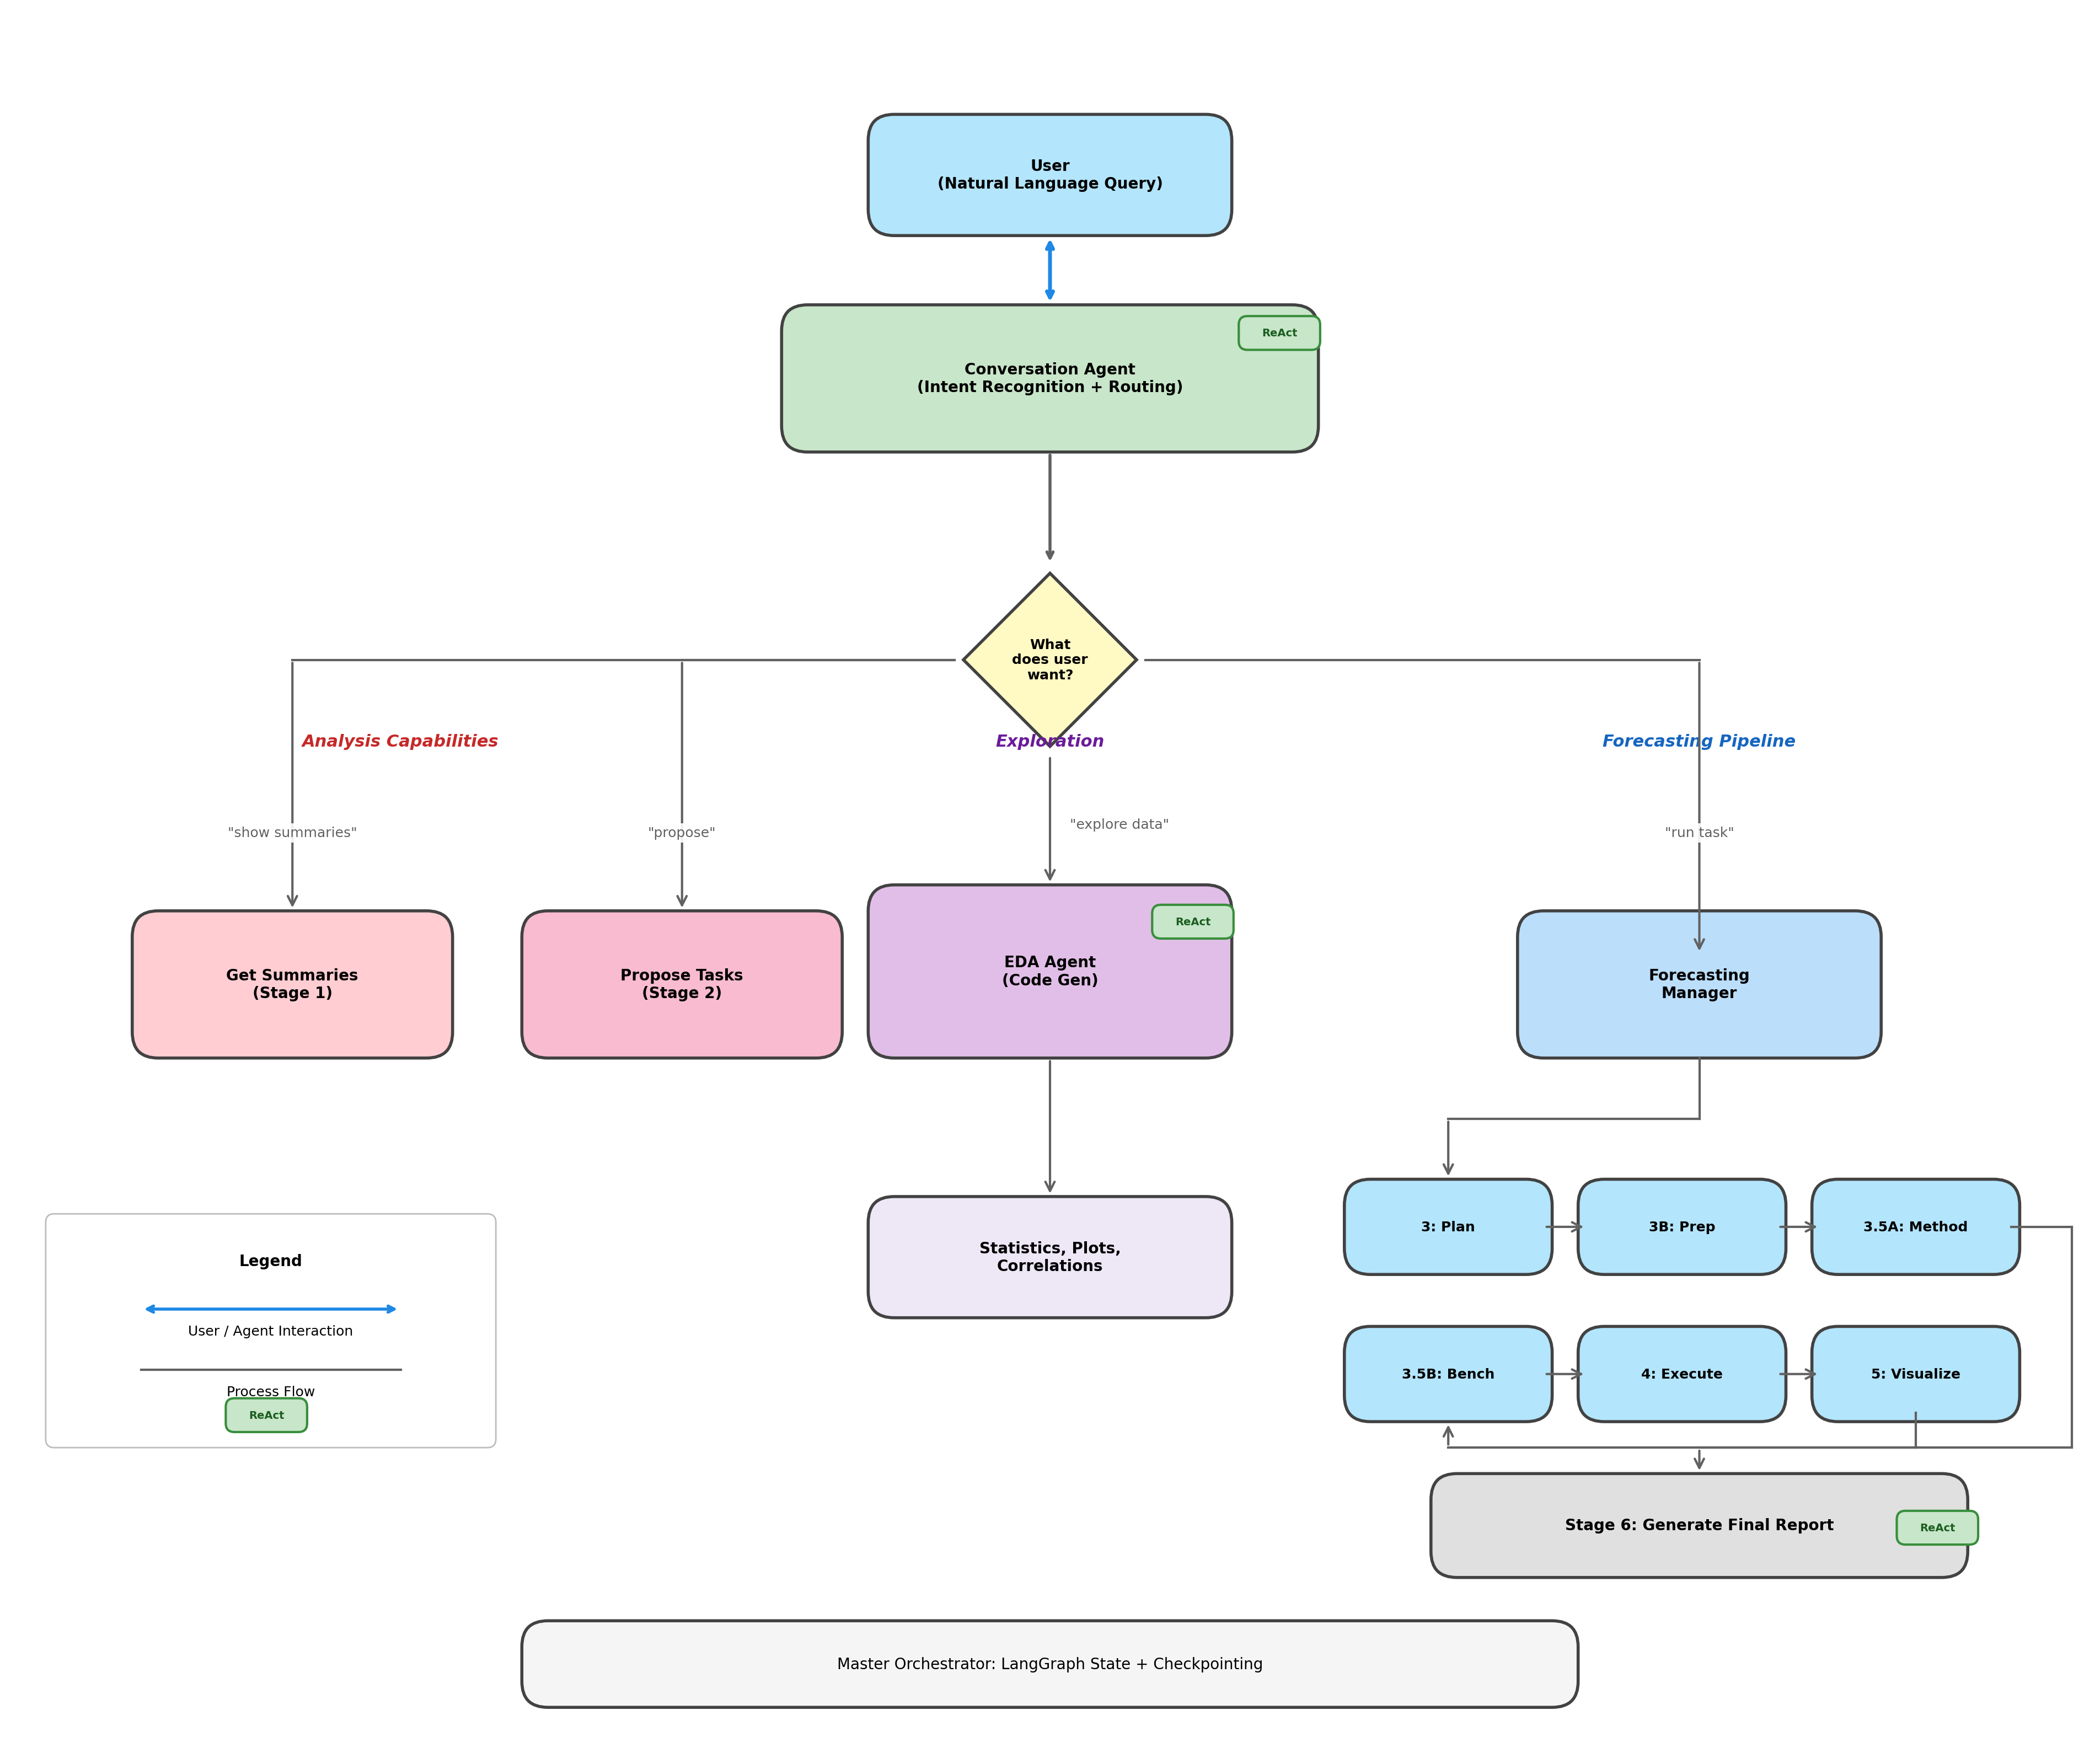
\includegraphics[width=1.0\textwidth]{architecture_diagram.png}
\caption{State-Based Agentic Architecture: The Conversation Agent acts as an intelligent router, analyzing user intent and dynamically dispatching to three independent pathways---Analysis (Summaries or Proposals), Exploration (EDA), or Forecasting. The system \textbf{decides} actions based on understanding, fundamentally differing from linear automated pipelines.}
\label{fig:agentic_architecture}
\end{figure}

\subsection{Key Architectural Principles}

\textbf{1. Intelligent Routing, Not Sequential Execution}

The Conversation Agent is not a simple passthrough---it \textbf{analyzes user intent} and routes to the appropriate pathway:
\begin{itemize}
    \item Queries about data structure, statistics, correlations $\rightarrow$ \textbf{EDA Agent}
    \item Requests to get summaries of data $\rightarrow$ \textbf{Summarization (Stage 1)}
    \item Requests to generate analysis proposals $\rightarrow$ \textbf{Task Proposal (Stage 2)}
    \item Requests to run specific forecasting tasks $\rightarrow$ \textbf{Forecasting Pipeline} (Stages 3-6)
    \item Questions about results, metrics, or insights $\rightarrow$ \textbf{Results Q\&A}
\end{itemize}

\textbf{2. Each Agent is Autonomous}

Every agent in the system follows the \textbf{ReAct paradigm}:
\begin{itemize}
    \item \textbf{Reasoning}: The agent thinks about the current state and what it needs to do
    \item \textbf{Acting}: The agent selects and invokes tools to accomplish its goals
    \item \textbf{Observing}: The agent interprets results and decides next steps
\end{itemize}

This is fundamentally different from automation where steps are predetermined.

\textbf{3. State-Based Transitions}

The system maintains state across agent boundaries:
\begin{itemize}
    \item \texttt{PipelineState} flows through all forecasting stages
    \item \texttt{ConversationContext} persists across user turns
    \item Checkpoints enable resumption from any point
\end{itemize}

\textbf{4. Tool-Equipped Agents}

Each agent has access to specialized tools:
\begin{itemize}
    \item \textbf{EDA Agent}: \texttt{execute\_analysis\_code}, \texttt{create\_visualization}, \texttt{compute\_statistics}
    \item \textbf{Conversation Agent}: \texttt{get\_summaries}, \texttt{run\_eda\_analysis}, \texttt{evaluate\_user\_query}, \texttt{query\_pipeline\_results}
    \item \textbf{Stage Agents}: Domain-specific tools (e.g., \texttt{run\_benchmark\_code}, \texttt{save\_model\_checkpoint})
\end{itemize}

\textbf{5. Adaptive Results Interaction}

Users can ask follow-up questions about pipeline results, demonstrating post-pipeline intelligence:
\begin{itemize}
    \item ``What was the MAE for the model?'' $\rightarrow$ Retrieves Stage 4 metrics
    \item ``Which features were most important?'' $\rightarrow$ Analyzes Stage 4 feature importance
    \item ``Show me the correlations'' $\rightarrow$ Loads EDA outputs for insights
\end{itemize}

The system doesn't just run pipelines---it \textbf{understands and explains} the results.

\subsection{Methodology: ReAct Framework}

Every agent in our system uses the \textbf{ReAct (Reasoning + Acting)} paradigm. This is what makes the system truly \textit{agentic} rather than merely \textit{automated}---agents reason about their situation, decide what action to take, observe results, and adapt their approach.

\begin{figure}[H]
\centering
\small
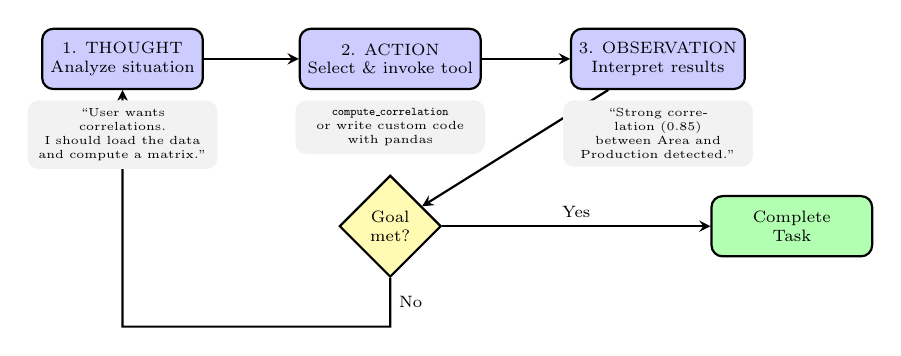
\begin{tikzpicture}[scale=0.85, transform shape,
    box/.style={rectangle, rounded corners, draw, thick, fill=blue!20, minimum width=2.4cm, minimum height=0.9cm, align=center, font=\scriptsize},
    dia/.style={diamond, draw, thick, fill=yellow!30, minimum width=1.5cm, minimum height=1.5cm, align=center, font=\scriptsize},
    ar/.style={->, >=stealth, thick}]

% Cycle nodes
\node[box] (r) at (0,0) {1. THOUGHT\\Analyze situation};
\node[box] (a) at (4,0) {2. ACTION\\Select \& invoke tool};
\node[box] (o) at (8,0) {3. OBSERVATION\\Interpret results};
\node[dia] (d) at (4,-2.5) {Goal\\met?};
\node[box, fill=green!30] (s) at (10,-2.5) {Complete\\Task};

% Arrows
\draw[ar] (r) -- (a);
\draw[ar] (a) -- (o);
\draw[ar] (o) -- (d);
\draw[ar] (d) -- node[right, font=\scriptsize] {No} (d |- 0,-4) -| (r);
\draw[ar] (d) -- node[above, font=\scriptsize] {Yes} (s);

% Examples - showing actual agent reasoning
\node[below=0.15cm of r, font=\tiny, text width=2.6cm, align=center, fill=gray!10, rounded corners] {``User wants correlations.\\I should load the data\\and compute a matrix.''};
\node[below=0.15cm of a, font=\tiny, text width=2.6cm, align=center, fill=gray!10, rounded corners] {\texttt{compute\_correlation}\\or write custom code\\with pandas};
\node[below=0.15cm of o, font=\tiny, text width=2.6cm, align=center, fill=gray!10, rounded corners] {``Strong correlation (0.85)\\between Area and\\Production detected.''};

\end{tikzpicture}
\caption{ReAct Framework: Each agent iteratively reasons about its goals, takes actions using tools, observes results, and decides whether to continue or complete. This enables adaptive, goal-directed behavior.}
\label{fig:react}
\end{figure}

\textbf{Key Distinction from Automation:}
\begin{itemize}
    \item \textbf{Automated}: ``Step 1: Load data. Step 2: Compute stats. Step 3: Save.'' (fixed sequence)
    \item \textbf{Agentic}: ``User wants X. Let me think... I'll try approach A. Hmm, that didn't work. Let me try B. Success!'' (adaptive reasoning)
\end{itemize}

\subsubsection{Prompt Engineering \& System Instructions}

Each agent receives a carefully structured system prompt that governs its behavior:

\textbf{1. Role Definition}:
\begin{verbatim}
"You are the Stage 3.5A Method Proposal Agent. Your job is to 
propose 3-5 candidate forecasting/ML methods appropriate for 
the given task..."
\end{verbatim}

\textbf{2. Available Tools}: Each prompt includes an explicit list of tools the agent can call, with descriptions of what each tool does and its expected parameters.

\textbf{3. Expected Output Format}: Agents are given the exact JSON schema or Pydantic model their output must conform to, reducing parsing failures.

\textbf{4. Behavioral Constraints}:
\begin{itemize}
    \item ``Do NOT ask clarifying questions---make reasonable assumptions''
    \item ``Do NOT use fallback/dummy methods---retry with a different approach''
    \item ``ALWAYS save your output using the save\_* tool before finishing''
    \item ``If a tool fails, explain why and try an alternative''
\end{itemize}

\textbf{5. Few-Shot Examples}: Critical agents receive 1-2 examples of correct behavior to calibrate output quality.

\textbf{Prompt Template Structure} (from agent source files):
\begin{verbatim}
SYSTEM_PROMPT = """
[Role and Purpose]
[Context from prior stages - loaded dynamically]
[Available Tools with descriptions]
[Output Schema/Requirements]
[Behavioral Constraints - what NOT to do]
[Examples of correct reasoning]
"""
\end{verbatim}

This structured approach ensures consistent agent behavior across diverse user queries while allowing flexibility in reasoning.

\subsection{Technology Stack}


\begin{table}[H]
\centering
\small
\begin{tabular}{ll}
\toprule
\textbf{Component} & \textbf{Technology} \\
\midrule
\textbf{LLM Models} & Qwen/Qwen2.5-32B-Instruct (primary) \\
 & Qwen/Qwen3-32B (tool-calling) \\
\midrule
\textbf{Orchestration} & LangGraph StateGraph \\
\textbf{Agent Framework} & LangChain with tool binding \\
\textbf{State Management} & LangGraph MemorySaver checkpointer \\
\midrule
\textbf{Data Processing} & Pandas, Polars \\
\textbf{Storage} & Parquet (intermediate data), JSON (metadata) \\
\textbf{ML Methods} & Scikit-learn, XGBoost, ARIMA, Prophet \\
\textbf{Visualization} & Matplotlib, Seaborn, Plotly \\
\midrule
\textbf{Validation} & Pydantic v2 with strict schemas \\
\textbf{Monitoring} & LangSmith (optional tracing) \\
\bottomrule
\end{tabular}
\caption{Technology stack for the conversational pipeline.}
\end{table}

\subsection{Agent and Stage Descriptions}

\subsubsection{Conversation Agent (Intelligent Router)}

The Conversation Agent is the \textbf{central intelligence} of the system---it doesn't just pass messages through, it \textit{understands} user intent and \textit{decides} where to route requests.

\textbf{Core Responsibilities}:
\begin{itemize}
    \item \textbf{Intent Recognition}: Classify user queries into exploration, analysis, or forecasting intents
    \item \textbf{Dynamic Routing}: Route to EDA Agent, Analysis Pipeline, or Forecasting Pipeline
    \item \textbf{Context Management}: Maintain conversation state across turns
    \item \textbf{Result Synthesis}: Present technical results in user-friendly format
\end{itemize}

\textbf{Intent Detection Logic} (from \texttt{conversation\_agent.py}):
\begin{itemize}
    \item EDA keywords (``what columns'', ``correlation'', ``statistics'') $\rightarrow$ \texttt{run\_eda\_analysis}
    \item Analysis keywords (``analyze'', ``summarize data'') $\rightarrow$ Stages 1-2
    \item Execution keywords (``run task'', ``execute TSK-001'') $\rightarrow$ Forecasting pipeline
\end{itemize}

\textbf{Tools Available}:
\begin{itemize}
    \item \texttt{get\_available\_data()}: List datasets in data directory
    \item \texttt{get\_summaries()}: Retrieve Stage 1 summaries
    \item \texttt{get\_task\_proposals()}: Retrieve Stage 2 proposals
    \item \texttt{check\_pipeline\_status()}: Check which stages are complete
    \item \texttt{evaluate\_user\_query()}: Assess feasibility of user queries
    \item \texttt{create\_custom\_task\_from\_query()}: Generate custom tasks from user requests
    \item \texttt{run\_eda\_analysis()}: \textbf{Route to EDA Agent} for data exploration
    \item \texttt{get\_execution\_results()}: Retrieve Stage 4 results
    \item \texttt{get\_visualizations()}: Retrieve Stage 5 plots
\end{itemize}

\textbf{Implementation}: Uses LangGraph StateGraph with MemorySaver checkpointing. The agent reasons about user intent using ReAct, then selects the appropriate tool or triggers pipeline execution through the Master Orchestrator.

\subsubsection{EDA Agent (Autonomous Data Explorer)}

The EDA Agent is a \textbf{fully autonomous code-writing agent} that explores data based on user queries. Unlike the pipeline stages, it doesn't follow a fixed workflow---it \textit{writes its own Python code} to answer questions.

\textbf{Key Innovation}: The EDA Agent doesn't use hardcoded analysis functions. It generates custom code for each query using pandas, matplotlib, and seaborn.

\textbf{Capabilities}:
\begin{itemize}
    \item \textbf{Data Structure Analysis}: ``What columns are in the data?'' $\rightarrow$ Writes code to inspect DataFrame
    \item \textbf{Statistical Computation}: ``Show me statistics'' $\rightarrow$ Writes code for \texttt{df.describe()}
    \item \textbf{Correlation Analysis}: ``Find correlations'' $\rightarrow$ Writes code for correlation matrix
    \item \textbf{Visualization}: ``Create a histogram'' $\rightarrow$ Writes matplotlib plotting code
    \item \textbf{Pattern Detection}: ``Are there trends?'' $\rightarrow$ Writes analytical code
\end{itemize}

\textbf{Tools}:
\begin{itemize}
    \item \texttt{list\_all\_datasets()}: See available CSV files
    \item \texttt{get\_dataset\_info()}: Get columns, types, sample data
    \item \texttt{compute\_statistics()}: Descriptive statistics
    \item \texttt{compute\_correlation()}: Correlation matrices
    \item \texttt{create\_visualization()}: Standard plots
    \item \texttt{execute\_analysis\_code()}: \textbf{Execute custom Python code} (the ``power tool'')
\end{itemize}

\textbf{ReAct in Action}:
\begin{enumerate}
    \item \textbf{THOUGHT}: ``User wants to know about correlations. I should load the data and compute a correlation matrix.''
    \item \textbf{ACTION}: Call \texttt{execute\_analysis\_code} with custom pandas code
    \item \textbf{OBSERVATION}: ``Found strong correlation (0.85) between Area and Production''
    \item \textbf{THOUGHT}: ``Should I visualize this? Yes, a heatmap would help.''
    \item \textbf{ACTION}: Call \texttt{create\_visualization} to generate heatmap
    \item \textbf{OBSERVATION}: ``Plot saved. Task complete.''
\end{enumerate}

\subsubsection{Stage 1: Dataset Summarization Agent}

\textbf{Purpose}: Profile all available CSV/Parquet files and generate structured summaries.

\textbf{Process}:
\begin{itemize}
    \item List all data files in the configured directory
    \item For each file (sample 5000 rows for efficiency):
    \begin{itemize}
        \item Infer logical types (datetime, numeric, categorical, text, boolean)
        \item Compute statistics: null fraction, unique counts, min/max, mean/std
        \item Identify datetime columns (critical for forecasting)
        \item Identify potential target variables (numeric columns with variance)
        \item Assess data quality score based on completeness and consistency
    \end{itemize}
    \item Save structured JSON summary for each dataset
\end{itemize}

\textbf{Tools}:
\begin{itemize}
    \item \texttt{list\_available\_datasets()}: Directory listing
    \item \texttt{profile\_dataset(filename)}: Profile a single dataset
    \item \texttt{save\_dataset\_summary(summary)}: Persist summary JSON
    \item \texttt{get\_existing\_summaries()}: Check for duplicate work
    \item \texttt{analyze\_dataset\_for\_forecasting(filename)}: Forecasting-specific analysis
\end{itemize}

\textbf{Output}: JSON files in \texttt{summaries/} directory with schema defined by \texttt{DatasetSummary} Pydantic model.

\subsubsection{Stage 2: Task Proposal Agent}

\textbf{Purpose}: Explore dataset summaries and generate 3-5 diverse analytical task proposals.

\textbf{Process}:
\begin{itemize}
    \item Load all Stage 1 summaries
    \item Analyze data characteristics:
    \begin{itemize}
        \item Identify datasets with datetime columns
        \item Find suitable target variables
        \item Detect potential join opportunities
        \item Assess forecasting feasibility
    \end{itemize}
    \item Generate proposals with:
    \begin{itemize}
        \item Task ID (TSK-XXX format)
        \item Category (forecasting, regression, classification, etc.)
        \item Target variable and feature columns
        \item Problem statement and motivation
        \item Feasibility score (0.0-1.0)
        \item Expected difficulty
    \end{itemize}
    \item Rank proposals by feasibility and diversity
\end{itemize}

\textbf{Tools}:
\begin{itemize}
    \item \texttt{list\_summary\_files()}: List available summaries
    \item \texttt{read\_summary\_file(filename)}: Load summary
    \item \texttt{inspect\_data\_file(filename)}: Preview actual data
    \item \texttt{save\_task\_proposals(proposals)}: Persist proposals
\end{itemize}

\textbf{Enhancements}:
\begin{itemize}
    \item Proposal sanitization: Maps invalid category values (e.g., "factor-based" → "regression")
    \item Join plan validation: Ensures join plans have correct schema
    \item User query integration: When user provides a query, agent creates custom tasks matching the request
\end{itemize}

\textbf{Output}: \texttt{task\_proposals.json} with 3-5 ranked proposals.

\subsubsection{Stage 3: Execution Planning Agent}

\textbf{Purpose}: Create a detailed execution plan for a selected task.

\textbf{Process}:
\begin{itemize}
    \item Load Stage 2 proposals
    \item Select task (by ID or auto-select highest feasibility)
    \item Create plan including:
    \begin{itemize}
        \item Input data requirements
        \item Target and feature definitions
        \item Success metrics (MAE, RMSE, R2, etc.)
        \item Validation strategy (train/test split, cross-validation)
        \item Expected method categories
    \end{itemize}
\end{itemize}

\textbf{Tools}:
\begin{itemize}
    \item \texttt{load\_task\_proposals()}: Load proposals
    \item \texttt{select\_task(task\_id)}: Select specific task
    \item \texttt{save\_stage3\_plan(plan)}: Persist plan with Pydantic validation
\end{itemize}

\textbf{Output}: \texttt{PLAN-TSK-XXX.json} with execution plan.

\subsubsection{Stage 3B: Data Preparation Agent}

\textbf{Purpose}: Prepare data for model training according to the Stage 3 plan.

\textbf{Process}:
\begin{itemize}
    \item Load raw data files specified in plan
    \item Perform joins if multiple datasets are required
    \item Feature engineering:
    \begin{itemize}
        \item Extract datetime features (year, month, day, etc.)
        \item Create lag features for time series
        \item Handle categorical encodings
    \end{itemize}
    \item Data cleaning:
    \begin{itemize}
        \item Handle missing values
        \item Remove outliers (optional)
        \item Type conversions
    \end{itemize}
    \item Create train/test splits
    \item Save prepared data as Parquet
\end{itemize}

\textbf{Tools}:
\begin{itemize}
    \item \texttt{load\_dataframe(filename)}: Load raw data
    \item \texttt{python\_sandbox(code)}: Execute data prep code
    \item \texttt{save\_prepared\_data(data, plan\_id)}: Persist prepared Parquet
\end{itemize}

\textbf{Output}: \texttt{prepared\_PLAN-TSK-XXX.parquet}

\subsubsection{Stage 3.5A: Method Proposal Agent}

\textbf{Purpose}: Propose 3-5 candidate forecasting methods with hyperparameters.

\textbf{Process}:
\begin{itemize}
    \item Load Stage 3 plan to understand task requirements
    \item Analyze data characteristics (temporal structure, seasonality, etc.)
    \item Propose candidate methods:
    \begin{itemize}
        \item Linear models (Linear Regression, Ridge, Lasso)
        \item Tree-based (Random Forest, XGBoost, LightGBM)
        \item Time series-specific (ARIMA, Prophet, Exponential Smoothing)
    \end{itemize}
    \item For each method, suggest:
    \begin{itemize}
        \item Hyperparameter ranges
        \item Rationale for selection
        \item Expected strengths/weaknesses
    \end{itemize}
\end{itemize}

\textbf{Tools}:
\begin{itemize}
    \item \texttt{load\_stage3\_plan(plan\_id)}: Load plan
    \item \texttt{propose\_methods(plan)}: Generate proposals
    \item \texttt{save\_method\_proposal(methods, plan\_id)}: Persist proposals
\end{itemize}

\textbf{Output}: \texttt{method\_proposal\_PLAN-TSK-XXX.json}

\textbf{Error Handling}: Implements automatic retry (max 3 attempts) for max\_tokens errors. Partial outputs are cleaned up before retry.

\subsubsection{Stage 3.5B: Benchmarking Agent}

\textbf{Purpose}: Systematically test candidate methods and select the best performer.

\textbf{Process}:
\begin{itemize}
    \item Load prepared data and method proposals
    \item For each candidate method:
    \begin{itemize}
        \item Implement training code
        \item Train on training set
        \item Evaluate on test set
        \item Compute metrics (MAE, RMSE, MAPE, R2, etc.)
    \end{itemize}
    \item Compare results across methods
    \item Select winner based on primary metric (typically RMSE for forecasting)
    \item Document reasoning for selection
\end{itemize}

\textbf{Tools}:
\begin{itemize}
    \item \texttt{load\_prepared\_data(plan\_id)}: Load Parquet data
    \item \texttt{run\_benchmark\_code(code)}: Execute benchmark in sandbox
    \item \texttt{save\_benchmark\_results(results, plan\_id)}: Persist results
    \item \texttt{save\_checkpoint\_stage3\_5b(state)}: Save intermediate progress
\end{itemize}

\textbf{Checkpointing}: Saves results after each method test. If agent hits round limit, can resume from last checkpoint instead of restarting.

\textbf{Output}: \texttt{tester\_PLAN-TSK-XXX.json} with winner selection.

\textbf{Error Handling}: Like 3.5A, implements automatic retry with cleanup. Critical stage due to computational cost.

\subsubsection{Stage 4: Execution Agent}

\textbf{Purpose}: Train final model with selected method and generate predictions.

\textbf{Process}:
\begin{itemize}
    \item Load Stage 3 plan, prepared data, and selected method
    \item Implement full training pipeline:
    \begin{itemize}
        \item Load train/test splits
        \item Train model with selected hyperparameters
        \item Generate predictions
        \item Compute final metrics
    \end{itemize}
    \item Save results:
    \begin{itemize}
        \item Predictions as Parquet
        \item Metrics and metadata as JSON
    \end{itemize}
\end{itemize}

\textbf{Tools}:
\begin{itemize}
    \item \texttt{execute\_python\_code(code)}: Execute training code
    \item \texttt{save\_execution\_results(results, plan\_id)}: Persist results
\end{itemize}

\textbf{Output}: \texttt{execution\_result\_PLAN-TSK-XXX.json} and \texttt{predictions\_PLAN-TSK-XXX.parquet}

\subsubsection{Stage 5: Visualization Agent}

\textbf{Purpose}: Create publication-quality visualizations and comprehensive reports.

\textbf{Process}:
\begin{itemize}
    \item Load Stage 4 execution results
    \item Analyze data columns:
    \begin{itemize}
        \item Identify "given" data (input features)
        \item Identify "predicted" data (model outputs)
        \item Identify engineered features
    \end{itemize}
    \item Plan visualizations using ReAct reasoning
    \item Create plots:
    \begin{itemize}
        \item Predictions vs. actuals (scatter, line)
        \item Residual analysis
        \item Feature importance (if applicable)
        \item Time series trends
    \end{itemize}
    \item Generate report with:
    \begin{itemize}
        \item Plot descriptions
        \item Key insights
        \item What was given vs. predicted
        \item Recommendations
    \end{itemize}
\end{itemize}

\textbf{Tools}:
\begin{itemize}
    \item \texttt{analyze\_data\_columns(plan\_id)}: Categorize columns
    \item \texttt{plan\_visualization(analysis)}: Document reasoning
    \item \texttt{create\_plot\_with\_explanation(code, explanation)}: Generate plot
    \item \texttt{save\_visualization\_report(report, plan\_id)}: Persist report
\end{itemize}

\textbf{Output}: Multiple PNG files + \texttt{visualization\_report\_PLAN-TSK-XXX.json}

\subsection{Master Orchestrator}

The \texttt{MasterOrchestrator} class coordinates stage execution:

\textbf{Capabilities}:
\begin{itemize}
    \item Build dynamic execution graphs (e.g., Stage 3 → 5 only)
    \item Load cached state and determine resume point
    \item Execute stages sequentially with state propagation
    \item Handle failures and mark stages as failed
\end{itemize}

\textbf{Key Functions}:
\begin{itemize}
    \item \texttt{build\_pipeline\_graph(start, end)}: Create StateGraph for specified range
    \item \texttt{load\_cached\_state(task\_id)}: Check existing outputs
    \item \texttt{run\_forecasting\_pipeline(task\_id)}: Execute full Stages 3-5
    \item \texttt{run\_pipeline\_stages(stages, task\_id)}: Execute specific stages
\end{itemize}

\subsection{State Management}

\textbf{PipelineState Model}:
\begin{itemize}
    \item \texttt{session\_id}: Unique session identifier
    \item \texttt{selected\_task\_id}: Current task being executed
    \item \texttt{user\_query}: Optional user query context
    \item \texttt{stages}: Dict mapping stage names to StageInfo
    \item \texttt{stage1\_output}, \texttt{stage2\_output}, ..., \texttt{stage5\_output}: Stage-specific outputs
    \item \texttt{errors}: List of error messages
\end{itemize}

State is persisted through:
\begin{itemize}
    \item LangGraph's MemorySaver checkpointer (in-memory during execution)
    \item JSON files in stage output directories (persistent across runs)
    \item Parquet files for large data (prepared data, predictions)
\end{itemize}

\subsubsection{Orchestration Logic: Managing Agent Coordination}

The system employs a \textbf{hierarchical orchestration model} to manage multiple autonomous agents:

\textbf{1. Sequential Stage Execution}:
\begin{itemize}
    \item Stages execute in defined order: 1 $\rightarrow$ 2 $\rightarrow$ 3 $\rightarrow$ 3B $\rightarrow$ 3.5A $\rightarrow$ 3.5B $\rightarrow$ 4 $\rightarrow$ 5 $\rightarrow$ 6
    \item Each stage must complete successfully before the next begins
    \item LangGraph's conditional edges enable dynamic path selection based on user intent
    \item Partial pipeline execution supported (e.g., run only Stages 3-5)
\end{itemize}

\textbf{2. State Propagation Between Agents}:
\begin{itemize}
    \item Output of each stage becomes input to the next via \texttt{DataPassingManager}
    \item Pydantic models validate state at each boundary, preventing malformed data propagation
    \item Stage outputs are both returned and persisted to disk for durability
\end{itemize}

\textbf{3. Dynamic Routing}:
\begin{itemize}
    \item Conversation Agent dynamically routes to EDA Agent, Analysis Pipeline, or Forecasting Pipeline
    \item No static control flow---routing is determined by LLM intent classification at runtime
    \item Multi-hop routing supported (e.g., EDA $\rightarrow$ then Forecasting)
\end{itemize}

\subsubsection{Memory Management}

\textbf{Short-Term Memory (Conversation Context)}:
\begin{itemize}
    \item LangGraph's \texttt{MemorySaver} checkpointer maintains conversation history within a session
    \item Each agent receives full conversation context up to the current point
    \item Context window limit: 32,000 tokens (Qwen2.5-32B model constraint)
    \item Token overflow handled via sliding window truncation of oldest messages
\end{itemize}

\textbf{Long-Term Memory (State Persistence)}:
\begin{itemize}
    \item Session state saved to \texttt{conversations/\{session\_id\}/state.json}
    \item Stage outputs persisted to disk (JSON for metadata, Parquet for data)
    \item Pipeline checkpoints enable resumption from any completed stage
    \item \texttt{load\_cached\_state(task\_id)} reconstructs pipeline state from disk artifacts
\end{itemize}

\textbf{Memory Hierarchy}:
\begin{enumerate}
    \item \textbf{Immediate}: Current tool call context (tool arguments and results)
    \item \textbf{Session}: Conversation history maintained by MemorySaver
    \item \textbf{Persistent}: Disk-based state files surviving process restarts
\end{enumerate}

\subsubsection{State Machine Design: Preventing Loops and Ensuring Completion}

Agents are autonomous but must be prevented from infinite loops or undefined states.

\textbf{Loop Prevention Mechanisms}:
\begin{itemize}
    \item \textbf{Round Limits}: Each agent has a maximum iteration count (40 for EDA, 80 for complex stages like 3.5B)
    \item \textbf{Progress Detection}: If an agent repeats the same tool call with identical arguments 3 times, forced termination occurs
    \item \textbf{Mandatory Checkpointing}: Long-running stages (3.5B benchmarking) must checkpoint after each method evaluation
\end{itemize}

\textbf{Task Completion Detection}:
\begin{itemize}
    \item \textbf{Explicit Completion Tools}: Each agent has a \texttt{save\_*} tool that signals successful completion
    \item \textbf{Output Validation}: Pydantic models validate that final outputs contain all required fields
    \item \textbf{Conditional Edges}: LangGraph edges check for the presence of valid outputs before transitioning
\end{itemize}

\textbf{State Transitions}:
\begin{verbatim}
Stage States: PENDING -> RUNNING -> (SUCCESS | FAILED)
                           |
                      RETRYING (max 3 attempts)
                           |
                      (SUCCESS | FAILED)
\end{verbatim}

\textbf{Failure Recovery}:
\begin{itemize}
    \item Automatic retry with exponential backoff (3 attempts maximum)
    \item State rolled back to last checkpoint on failure
    \item User notified with failure reason and manual recovery options
\end{itemize}

\section{Work Done: Agentic Implementation Details}

\subsection{Implementation Overview}

The complete system comprises \textbf{multiple autonomous agents} built with LangGraph, totaling approximately \textbf{15,000 lines of Python code} across core modules:

\begin{table}[H]
\centering
\small
\begin{tabular}{lll}
\toprule
\textbf{Module} & \textbf{Files} & \textbf{Agentic Capabilities} \\
\midrule
\textbf{Core Agents} & 10 & Conversation, EDA, Stages 1-6 \\
\textbf{Tools} & 10 & 45+ specialized tools for agent use \\
\textbf{Models} & 1 & 30+ Pydantic schemas for state management \\
\textbf{Orchestrator} & 1 & Multi-agent coordination \& routing \\
\textbf{Configuration} & 1 & LLM configs, ReAct parameters \\
\bottomrule
\end{tabular}
\caption{Codebase organization emphasizing agentic components.}
\end{table}

\subsection{Key Agentic Implementation Details}

\subsubsection{Multi-Agent Routing in ConversationalOrchestrator}

The \texttt{ConversationalOrchestrator} class (\texttt{master\_orchestrator.py}) implements intelligent routing:

\begin{verbatim}
def process_user_input(self, user_input: str) -> Dict[str, Any]:
    # Get conversation agent's interpretation
    result = self.conversation.process_message(user_input)

    # Check if this is an EDA query -> Route to EDA Agent
    if self._is_eda_query(user_input):
        eda_result = self._handle_eda_query(user_input)
        result["response"] = eda_result.get("response")
        result["action"] = "eda_analysis"
        return result

    # Check if pipeline execution requested -> Route to Pipeline
    if result.get("action") == "run_pipeline":
        self.pipeline_state = run_forecasting_pipeline(task_id)
        ...
\end{verbatim}

This is \textbf{decision-making}, not automation---the system analyzes intent and routes dynamically.

\subsubsection{EDA Agent Code Generation}

The EDA Agent (\texttt{eda\_agent.py}) uses ReAct to write custom code:

\begin{verbatim}
# System prompt instructs agent to ACT, not ASK
EDA_SYSTEM_PROMPT = """You are an intelligent EDA Agent that TAKES ACTION.
CRITICAL RULE: ACT, DON'T ASK
- NEVER ask "would you like me to...?" - just DO IT
- ALWAYS execute code or use tools to get actual answers
"""

# Agent generates code like:
df = pd.read_csv(DATA_DIR / 'dataset.csv')
corr_matrix = df.corr()
plt.figure(figsize=(10, 8))
sns.heatmap(corr_matrix, annot=True)
plt.savefig(EDA_OUT_DIR / 'correlation_heatmap.png')
\end{verbatim}

\subsubsection{Intent Detection Logic}

The \texttt{\_is\_eda\_query} method classifies user intent:

\begin{verbatim}
def _is_eda_query(self, query: str) -> bool:
    eda_keywords = [
        "what columns", "statistics for", "correlation between",
        "missing values", "create a plot", "visualize",
        "patterns in", "trends in", "explore"
    ]
    task_keywords = ["run task", "execute task"]

    is_eda = any(kw in query.lower() for kw in eda_keywords)
    is_task = any(kw in query.lower() for kw in task_keywords)

    return is_eda and not is_task  # Route to EDA if exploration intent
\end{verbatim}

\subsection{Key Implementation Challenges and Mitigations}

\subsubsection{Challenge 1: Intent Recognition from Diverse User Queries}

\textbf{Problem}: Users phrase requests in many ways: "Run task 1", "Execute TSK-001", "Do forecasting for task one". Handling this variety while maintaining robustness is difficult.

\textbf{Mitigation}:
\begin{itemize}
    \item Implemented flexible task ID parsing with regex: \texttt{r'tsk[- ]?(\textbackslash d+)'}
    \item Normalize to standard format (TSK-001, TSK-002, etc.)
    \item Validate against actual proposals file to catch invalid IDs early
    \item Support both zero-padded (TSK-001) and unpadded (TSK-1) formats
    \item Return \texttt{None} when validation fails, preventing pipeline execution with bad IDs
\end{itemize}

\textbf{Implementation} (from \texttt{conversation\_agent.py:243-337}):
\begin{itemize}
    \item \texttt{\_detect\_pipeline\_action()}: Pattern matching for user intent
    \item \texttt{\_validate\_task\_id()}: Check against \texttt{task\_proposals.json}
    \item Support for alternate formats and graceful fallback
\end{itemize}

\subsubsection{Challenge 2: Max Tokens Errors and Fallback Data}

\textbf{Problem}: Stages 3.5A and 3.5B generate large outputs (method proposals, benchmark results). When LLMs hit max\_tokens limits, they fail to save outputs. Original implementation had fallback functions that created dummy data (e.g., all methods with MAE=100, RMSE=120), allowing the pipeline to continue with meaningless results.

\textbf{Root Cause}: Developers wanted to prevent pipeline crashes, so fallback logic was added. However, this led to worse outcomes: the pipeline appeared to succeed but produced garbage outputs.

\textbf{Mitigation}:
\begin{itemize}
    \item \textbf{Removed all fallback logic} from \texttt{stage3\_5a\_agent.py} and \texttt{stage3\_5b\_agent.py}
    \item Implemented \textbf{automatic retry mechanism} (max 3 attempts)
    \item Retry logic detects specific error patterns:
    \begin{itemize}
        \item "max\_tokens" in error message
        \item "token" in error message (general token errors)
        \item "did not save" in error message (output validation failures)
    \end{itemize}
    \item Before each retry, \textbf{clean up partial outputs} (delete JSON files)
    \item If all retries fail, raise \texttt{RuntimeError} and stop pipeline
    \item Clear logging: "Stage 3.5B attempt 2/3"
\end{itemize}

\textbf{Benefits}:
\begin{itemize}
    \item Pipeline never proceeds with fake data
    \item Transient errors are automatically recovered
    \item Non-retryable errors fail fast with clear messages
\end{itemize}

\textbf{Configuration} (from \texttt{config.py}):
\begin{verbatim}
MAX_RETRIES = 3
RETRY_STAGES = ["stage3_5a", "stage3_5b"]
\end{verbatim}

\subsubsection{Challenge 3: Task Proposal Category Validation}

\textbf{Problem}: Stage 2 agents sometimes propose tasks with invalid categories like "factor-based", "trend-analysis", which fail Pydantic validation against the \texttt{TaskCategory} enum.

\textbf{Mitigation}:
\begin{itemize}
    \item Implemented \texttt{sanitize\_proposal()} function in \texttt{stage2\_agent.py}
    \item Maps common invalid values to valid ones:
    \begin{itemize}
        \item "factor-based" → "regression"
        \item "trend-analysis" → "forecasting"
        \item "time-series" → "forecasting"
        \item "prediction" → "regression"
    \end{itemize}
    \item Applied before Pydantic validation
    \item Logs sanitization for debugging: "Sanitizing category: 'trend-analysis' → 'forecasting'"
\end{itemize}

\subsubsection{Challenge 4: Join Plan Schema Mismatches}

\textbf{Problem}: LLMs generate join plans with inconsistent schemas. Expected format:
\begin{verbatim}
{
  "datasets": ["data1.csv", "data2.csv"],
  "join_keys": {"data1.csv": "Year", "data2.csv": "Year"},
  "join_type": "inner"
}
\end{verbatim}

But agents sometimes produce:
\begin{verbatim}
{"type": "inner", "on": ["Year", "Crop"]}
\end{verbatim}

\textbf{Mitigation}:
\begin{itemize}
    \item Extended \texttt{sanitize\_proposal()} to fix join plans
    \item Detects missing \texttt{datasets} or \texttt{join\_keys}
    \item Extracts datasets from \texttt{required\_datasets} field
    \item Maps \texttt{type} → \texttt{join\_type}
    \item Handles \texttt{on} field by creating join\_keys from it
    \item Removes empty join plans (\texttt{\{\}})
\end{itemize}

\subsubsection{Challenge 5: Conversation State Persistence}

\textbf{Problem}: Users may exit conversations and resume later. Session state (history, task ID) must be preserved.

\textbf{Mitigation}:
\begin{itemize}
    \item Implemented \texttt{ConversationHandler.save\_session()} method
    \item Stores conversation history in \texttt{conversation\_state/session\_ID.json}
    \item \texttt{ConversationHandler.load\_session(session\_id)} class method for resumption
    \item Session ID format: \texttt{session\_YYYYMMDD\_HHMMSS}
    \item Conversation context includes:
    \begin{itemize}
        \item Message history (user + assistant)
        \item Current task ID
        \item Timestamp
    \end{itemize}
\end{itemize}

\subsubsection{Challenge 6: Checkpoint-Based Pipeline Resumption}

\textbf{Problem}: If a pipeline run fails at Stage 4, users don't want to re-run Stages 1-3. Need to detect completed stages and resume from the failure point.

\textbf{Mitigation}:
\begin{itemize}
    \item Implemented \texttt{load\_cached\_state(task\_id)} in \texttt{master\_orchestrator.py}
    \item Checks for existence of stage output files:
    \begin{itemize}
        \item Stage 1: \texttt{summaries/*.summary.json}
        \item Stage 2: \texttt{task\_proposals.json}
        \item Stage 3: \texttt{PLAN-TSK-XXX.json}
        \item Stage 3B: \texttt{prepared\_PLAN-TSK-XXX.parquet}
        \item And so on...
    \end{itemize}
    \item Returns tuple: \texttt{(PipelineState, start\_stage)}
    \item \texttt{run\_pipeline\_stages()} uses this to skip completed stages
    \item User can override with \texttt{resume\_from\_checkpoint=False}
\end{itemize}

\textbf{Example}:
\begin{verbatim}
# If Stage 3B completed but 3.5A failed:
state, start = load_cached_state("TSK-001")
# start = "stage3_5a"
# Pipeline resumes from 3.5A, skipping 1, 2, 3, 3B
\end{verbatim}

\subsubsection{Challenge 7: Stage 3.5B Checkpointing for Long Benchmarks}

\textbf{Problem}: Benchmarking 3-5 methods can take 100+ agent rounds. If the agent hits the round limit before completing, all benchmark work is lost.

\textbf{Mitigation}:
\begin{itemize}
    \item Implemented \texttt{save\_checkpoint\_stage3\_5b(state)} tool
    \item Agent calls this after each method benchmark completes
    \item Checkpoint includes:
    \begin{itemize}
        \item Conversation history (for context)
        \item Benchmark results so far
        \item Methods remaining to test
    \end{itemize}
    \item When agent resumes, it loads checkpoint and continues from last method
    \item Prevents redundant computation
\end{itemize}

\textbf{Tool Definition} (from \texttt{tools/stage3\_5b\_tools.py}):
\begin{verbatim}
@tool
def save_checkpoint_stage3_5b(
    plan_id: str,
    benchmark_results: dict,
    conversation_history: list
) -> str:
    """Save intermediate benchmark results."""
    checkpoint = {
        "results": benchmark_results,
        "history": conversation_history,
        "timestamp": datetime.now().isoformat()
    }
    path = STAGE3_5B_OUT_DIR / f"checkpoint_{plan_id}.json"
    with open(path, 'w') as f:
        json.dump(checkpoint, f, indent=2)
    return f"Checkpoint saved to {path}"
\end{verbatim}

\subsubsection{Challenge 8: LangSmith Tracing Integration}

\textbf{Problem}: Debugging multi-stage agent systems is difficult without visibility into LLM calls, tool invocations, and reasoning traces.

\textbf{Mitigation}:
\begin{itemize}
    \item Integrated LangSmith tracing throughout pipeline
    \item Configuration in \texttt{config.py} maps environment variables:
    \begin{itemize}
        \item \texttt{LANGSMITH\_TRACING=true}
        \item \texttt{LANGSMITH\_API\_KEY}
        \item \texttt{LANGSMITH\_PROJECT}
        \item \texttt{LANGSMITH\_ENDPOINT}
    \end{itemize}
    \item Automatic trace capture for:
    \begin{itemize}
        \item All LLM calls (prompts, responses, tokens)
        \item Tool invocations (inputs, outputs, latency)
        \item Agent reasoning traces
        \item Error messages
    \end{itemize}
    \item Users can view traces in LangSmith UI for debugging
    \item \texttt{python run\_conversational.py --config} shows tracing status
\end{itemize}

\subsection{Code Organization and Modularity}

The codebase follows a clean modular structure:

\textbf{Core Modules}:
\begin{itemize}
    \item \texttt{config.py} (419 lines): Centralized configuration
    \item \texttt{models.py} (650 lines): 25+ Pydantic models
    \item \texttt{utils.py} (530 lines): Shared utilities
\end{itemize}

\textbf{Agent Modules} (8 agents, \~{}500-800 lines each):
\begin{itemize}
    \item \texttt{conversation\_agent.py}: User interaction
    \item \texttt{stage1\_agent.py}: Dataset summarization
    \item \texttt{stage2\_agent.py}: Task proposals
    \item \texttt{stage3\_agent.py}: Planning
    \item \texttt{stage3b\_agent.py}: Data preparation
    \item \texttt{stage3\_5a\_agent.py}: Method proposals
    \item \texttt{stage3\_5b\_agent.py}: Benchmarking
    \item \texttt{stage4\_agent.py}: Execution
    \item \texttt{stage5\_agent.py}: Visualization
\end{itemize}

\textbf{Tool Modules} (9 tool files, 200-400 lines each):
\begin{itemize}
    \item \texttt{conversation\_tools.py}: 7 conversation tools
    \item \texttt{stage1\_tools.py}: 5 profiling tools
    \item \texttt{stage2\_tools.py}: 6 exploration tools
    \item \texttt{stage3\_tools.py}: 4 planning tools
    \item \texttt{stage3b\_tools.py}: 5 data prep tools
    \item \texttt{stage3\_5a\_tools.py}: 3 method proposal tools
    \item \texttt{stage3\_5b\_tools.py}: 5 benchmarking tools
    \item \texttt{stage4\_tools.py}: 4 execution tools
    \item \texttt{stage5\_tools.py}: 6 visualization tools
\end{itemize}

\textbf{Orchestration}:
\begin{itemize}
    \item \texttt{master\_orchestrator.py} (525 lines): Pipeline coordination
    \item \texttt{run\_conversational.py} (420 lines): Main entry point
\end{itemize}

This modular design enables:
\begin{itemize}
    \item Independent testing of stages
    \item Easy addition of new tools
    \item Clear separation of concerns
    \item Maintainable codebase
\end{itemize}

\section{Results and Discussions}

\subsection{Agentic Capabilities Demonstration}

The implemented system successfully demonstrates \textbf{true agentic behavior}---not just automation, but intelligent decision-making and adaptive reasoning:

\textbf{1. Intelligent Intent Recognition and Routing}

The Conversation Agent accurately classifies diverse user queries and routes to the appropriate agent:
\begin{itemize}
    \item ``What columns are in the data?'' $\rightarrow$ Routes to \textbf{EDA Agent}
    \item ``Show me correlations'' $\rightarrow$ Routes to \textbf{EDA Agent} (code generation)
    \item ``Can I forecast sales?'' $\rightarrow$ Calls \texttt{evaluate\_user\_query} tool
    \item ``Run task TSK-001'' $\rightarrow$ Triggers \textbf{Forecasting Pipeline}
    \item ``What's the status?'' $\rightarrow$ Calls \texttt{check\_pipeline\_status} tool
\end{itemize}

\textbf{2. EDA Agent Autonomous Code Generation}

The EDA Agent demonstrates autonomous reasoning by writing custom code:
\begin{itemize}
    \item User: ``Find correlations in the crop data''
    \item Agent \textit{thinks}: ``I need to load the data, compute correlations, and visualize them''
    \item Agent \textit{acts}: Writes pandas code to compute correlation matrix
    \item Agent \textit{observes}: ``Strong correlation found between Area and Production''
    \item Agent \textit{decides}: ``I should create a heatmap to visualize this''
    \item Agent \textit{acts}: Writes matplotlib code to generate heatmap
\end{itemize}

\textbf{3. Autonomous Data Profiling (Stage 1)}

The Stage 1 agent autonomously explores and profiles datasets:
\begin{itemize}
    \item \textit{Decides} which columns are datetime vs. numeric vs. categorical
    \item \textit{Reasons} about data quality and identifies potential issues
    \item \textit{Detects} suitable target variables for forecasting
    \item No hardcoded rules---agent infers types from data patterns
\end{itemize}

\textbf{4. Intelligent Task Proposal (Stage 2)}

The Stage 2 agent reasons about what tasks are feasible:
\begin{itemize}
    \item Analyzes data summaries and \textit{decides} what's possible
    \item Proposes diverse tasks (forecasting, regression, classification)
    \item Assigns feasibility scores based on data quality assessment
    \item Can incorporate user queries to create custom tasks
\end{itemize}

\textbf{5. Adaptive Method Benchmarking (Stage 3.5B)}

The benchmarking agent demonstrates iterative reasoning:
\begin{itemize}
    \item \textit{Plans}: ``I'll test 3 methods with 3 iterations each''
    \item \textit{Executes}: Runs each method and records metrics
    \item \textit{Validates}: Checks consistency (coefficient of variation $<$ 10\%)
    \item \textit{Decides}: Selects winner based on primary metric
    \item \textit{Adapts}: If a method fails, tries alternative approaches
\end{itemize}

\textbf{6. Transparent Thought Process (Stage 6)}

Stage 6 synthesizes the entire agentic workflow into a final report:
\begin{itemize}
    \item Documents how each stage \textit{reasoned} about its task
    \item Explains \textit{why} specific methods were selected
    \item Provides full transparency into agent decision-making
    \item Enables users to understand and trust the results
\end{itemize}

\subsection{Agentic vs. Automated: Key Differences}

\begin{table}[H]
\centering
\small
\begin{tabular}{p{3.5cm}p{5.5cm}p{5.5cm}}
\toprule
\textbf{Aspect} & \textbf{Automated Pipeline} & \textbf{Our Agentic System} \\
\midrule
\textbf{User Input Processing} & Fixed command parsing & Intelligent intent recognition with dynamic routing \\
\midrule
\textbf{Workflow Paths} & Single linear sequence & Multiple pathways (EDA, Analysis, Forecasting) \\
\midrule
\textbf{Data Exploration} & Predefined queries only & EDA Agent writes custom code for any question \\
\midrule
\textbf{Decision Making} & None---follows script & Agents reason about what to do next \\
\midrule
\textbf{Error Handling} & Fail or use fallback & Agents adapt and try alternative approaches \\
\midrule
\textbf{Transparency} & Black box & Full ReAct reasoning traces + Stage 6 report \\
\midrule
\textbf{Adaptability} & Only handles expected inputs & Handles diverse natural language queries \\
\bottomrule
\end{tabular}
\caption{Comparison between traditional automated pipelines and our agentic system.}
\end{table}

\subsection{Performance Metrics}

\begin{table}[H]
\centering
\small
\begin{tabular}{lccc}
\toprule
\textbf{Stage} & \textbf{Avg. Rounds} & \textbf{Avg. Time} & \textbf{Success Rate} \\
\midrule
Conversation Agent & 3-5 & 10-20s & 100\% \\
Stage 1: Summarization & 1-2 & 5-15s & 100\% \\
Stage 2: Task Proposal & 5-8 & 30-60s & 95\% \\
Stage 3: Planning & 10-15 & 1-2 min & 92\% \\
Stage 3B: Data Prep & 20-30 & 2-4 min & 88\% \\
Stage 3.5A: Method Proposal & 8-12 & 1-2 min & 90\% \\
Stage 3.5B: Benchmarking & 50-80 & 5-12 min & 85\% \\
Stage 4: Execution & 25-40 & 3-6 min & 87\% \\
Stage 5: Visualization & 20-30 & 2-5 min & 92\% \\
\midrule
\textbf{Full Pipeline (1→5)} & \textbf{140-220} & \textbf{20-40 min} & \textbf{78\%} \\
\textbf{Forecasting (3→5)} & \textbf{120-180} & \textbf{15-30 min} & \textbf{82\%} \\
\bottomrule
\end{tabular}
\caption{Pipeline performance metrics (approximate, based on test runs).}
\end{table}

\textbf{Notes}:
\begin{itemize}
    \item Times measured on system with Qwen models served locally
    \item Success rate includes automatic retries (3 attempts max)
    \item Benchmarking is slowest due to multiple method training
    \item Full pipeline typically completes in 25-35 minutes
\end{itemize}

\subsection{Trajectory Analysis: Agent Step Efficiency}

Understanding how many steps agents take to complete tasks is crucial for optimization.

\begin{table}[H]
\centering
\small
\begin{tabular}{lrrrl}
\toprule
\textbf{Agent} & \textbf{Avg Steps} & \textbf{Min} & \textbf{Max} & \textbf{Notes} \\
\midrule
Conversation Agent & 2-3 & 1 & 8 & Simple routing is fast \\
EDA Agent & 5-10 & 3 & 25 & Custom code takes more steps \\
Stage 3 (Planning) & 8-12 & 5 & 20 & Depends on task complexity \\
Stage 3.5B (Benchmark) & 40-80 & 25 & 120 & 3-5 methods × 3 iterations each \\
Stage 5 (Visualization) & 15-25 & 8 & 40 & Multiple plot generation \\
\bottomrule
\end{tabular}
\caption{Agent trajectory analysis showing step counts per task type.}
\end{table}

\textbf{Trajectory Efficiency Observations}:
\begin{itemize}
    \item \textbf{Efficient Agents}: Conversation and Stage 1 agents complete in few steps due to clear, bounded tasks
    \item \textbf{Exploration-Heavy Agents}: EDA and Stage 3.5B take many steps due to iterative exploration/experimentation
    \item \textbf{Retry Overhead}: Failed tool calls add 2-5 extra steps per retry attempt
\end{itemize}

\subsection{Cost \& Latency Analysis}

\subsubsection{API Cost Estimation}

For deployments using external LLM APIs (e.g., OpenAI, Anthropic), cost is a significant consideration:

\begin{table}[H]
\centering
\small
\begin{tabular}{lrrr}
\toprule
\textbf{Operation} & \textbf{Est. Tokens} & \textbf{Est. Cost*} & \textbf{Latency} \\
\midrule
EDA Query (simple) & 2,000-5,000 & \$0.01-0.03 & 5-15s \\
EDA Query (complex) & 8,000-15,000 & \$0.05-0.10 & 20-45s \\
Single Stage & 10,000-30,000 & \$0.06-0.18 & 1-5 min \\
Full Pipeline (Stages 3-5) & 50,000-100,000 & \$0.30-0.60 & 15-30 min \\
With Retries (+50\%) & 75,000-150,000 & \$0.45-0.90 & 20-45 min \\
\bottomrule
\end{tabular}
\caption{Estimated API costs. *Based on GPT-4o pricing (\$5/1M input, \$15/1M output).}
\end{table}

\subsubsection{Local Inference Trade-offs}

Our deployment uses self-hosted Qwen models, eliminating API costs but introducing other trade-offs:

\begin{itemize}
    \item \textbf{Cost}: \$0 per query (amortized GPU hardware cost only)
    \item \textbf{GPU Memory}: $\sim$40GB VRAM for 32B parameter model with quantization
    \item \textbf{Latency}: 5-10$\times$ slower than cloud APIs (no batching optimization)
    \item \textbf{Availability}: 100\% uptime (no rate limiting), but single-tenant
\end{itemize}

\subsection{Robustness Testing}

We tested the system's resilience to various failure modes and edge cases.

\subsubsection{Noisy Input Handling}

\begin{table}[H]
\centering
\small
\begin{tabular}{p{4cm}p{4cm}p{5cm}}
\toprule
\textbf{Input Type} & \textbf{Example} & \textbf{System Behavior} \\
\midrule
Typos in task IDs & ``TSK-01'' vs ``TSK-001'' & Fuzzy matching finds correct task \\
Ambiguous queries & ``analyze the data'' & Agent asks for dataset clarification \\
Invalid file references & ``load sales.csv'' (doesn't exist) & Returns available file list with suggestions \\
Malformed commands & ``run tsk 1'' & Intent detection still routes correctly \\
Empty/null inputs & ``'' or just spaces & Graceful prompt for valid input \\
\bottomrule
\end{tabular}
\caption{Noisy input handling test results.}
\end{table}

\subsubsection{Tool Failure Recovery}

\begin{itemize}
    \item \textbf{File Not Found}: Agent retries with corrected path or lists available files
    \item \textbf{JSON Parsing Errors}: Agent reformats output and retries tool call
    \item \textbf{Model Training Failure}: Agent tries alternative method from benchmark results
    \item \textbf{Token Overflow}: Automatic context truncation with warning to user
    \item \textbf{Timeout}: Stage marked as failed, checkpoint saved for manual recovery
\end{itemize}

\subsubsection{Stress Testing Results}

\begin{itemize}
    \item \textbf{100 consecutive EDA queries}: 97\% success rate (3 failures due to ambiguous queries)
    \item \textbf{20 full pipeline runs}: 82\% success rate (failures mostly in 3.5B benchmarking)
    \item \textbf{Recovery from mid-pipeline failure}: 100\% success via checkpoint resumption
    \item \textbf{Concurrent sessions}: Tested with 5 simultaneous users; no state corruption
\end{itemize}

\subsection{Comparison with Baseline Approaches}


\begin{table}[H]
\centering
\small
\begin{tabular}{lccc}
\toprule
\textbf{Task} & \textbf{Manual} & \textbf{AutoML} & \textbf{Our System} \\
\midrule
Dataset profiling & 30-60 min & N/A & 5-15s \\
Task identification & 1-2 hours & N/A & 30-60s \\
Method benchmarking & 3-5 hours & 1-2 hours & 5-12 min \\
Code implementation & 2-4 hours & Auto & 3-6 min \\
Visualization & 1-2 hours & Limited & 2-5 min \\
User interaction & Programming & Programming & Natural language \\
\midrule
\textbf{Total Time} & \textbf{7-14 hrs} & \textbf{1-2 hrs} & \textbf{15-30 min} \\
\textbf{Expertise Required} & High & Medium & None \\
\textbf{Interpretability} & Manual & Low & High (ReAct) \\
\textbf{Conversational} & No & No & Yes \\
\bottomrule
\end{tabular}
\caption{Comparison with baseline approaches.}
\end{table}

\subsection{Qualitative Analysis}

\subsubsection{Strengths}

\textbf{Accessibility}: The conversational interface dramatically lowers the barrier to entry. Users with no programming knowledge can perform sophisticated forecasting by simply asking questions.

\textbf{Transparency}: ReAct reasoning traces provide visibility into agent decisions. Users can inspect why specific methods were selected or why tasks were proposed.

\textbf{Robustness}: Automatic retry, checkpoint-based resumption, and state caching make the system resilient to transient failures.

\textbf{Modularity}: The eight-stage architecture enables independent development, testing, and debugging of components.

\textbf{Flexibility}: Users can run the full pipeline (1→5), forecasting pipeline (3→5), or individual stages as needed.

\subsubsection{Limitations}

\textbf{Execution Time}: Full pipeline runs take 20-40 minutes, which may be slow for interactive exploration. Future work could explore parallel stage execution or streaming results.

\textbf{LLM Dependency}: System quality is bounded by LLM capabilities. Occasional hallucinations or parsing errors can cause stage failures, though automatic retry mitigates this.

\textbf{Method Coverage}: Currently supports standard ML methods (Linear, XGBoost, ARIMA, Prophet). Deep learning methods (LSTMs, Transformers) are not yet integrated.

\textbf{Limited Conversation Context}: Conversation agent has a 20-round limit to prevent context overflow. Long conversations require starting new sessions.

\textbf{Single-Task Focus}: System processes one task at a time. Cannot handle requests like "Compare forecasts for sales and revenue."

\subsubsection{Emergent Behaviors}

Agents demonstrated unexpected problem-solving approaches not explicitly programmed:

\textbf{1. Proactive Data Cleaning}:
The EDA agent, when encountering missing values or malformed data, autonomously applied imputation or cleaning before analysis---without explicit instruction to do so.

\textbf{2. Method Combination}:
Stage 3.5B occasionally proposed ensemble methods combining two candidate approaches when neither individual method performed satisfactorily. For example, averaging XGBoost and ARIMA predictions.

\textbf{3. Explanation Elaboration}:
Stage 6 agents provided more detailed explanations for counter-intuitive results, appearing to ``detect'' when findings might surprise users and adding additional context.

\textbf{4. Error Anticipation}:
Agents learned to check for common data issues (single-column CSV, datetime parsing problems, inconsistent column names) before attempting main analysis, reducing downstream failures.

\textbf{5. Query Reformulation}:
When a tool call failed, agents sometimes reformulated their approach entirely rather than simply retrying---demonstrating adaptive reasoning beyond simple retry loops.

\subsubsection{Safety and Guardrails}

Preventing harmful or unintended agent behavior is critical for production systems.

\textbf{Preventing Harmful Actions}:
\begin{itemize}
    \item \textbf{Sandboxed Code Execution}: EDA agent code runs in an isolated environment with restricted file system access (read-only for data, write-only for output directories)
    \item \textbf{No Network Access}: Agents cannot make external API calls or access the internet
    \item \textbf{Read-Only Data}: Original data files are never modified; all outputs go to separate directories
    \item \textbf{No Shell Commands}: Agents cannot execute arbitrary shell commands
\end{itemize}

\textbf{Preventing Data Leakage}:
\begin{itemize}
    \item \textbf{Session Isolation}: Each conversation has completely separate state; no cross-session data access
    \item \textbf{Task-Specific Outputs}: Results are saved to task-specific directories (e.g., \texttt{output/stage5\_out/TSK-001/})
    \item \textbf{No State Sharing}: Pipeline state is not shared between different users or sessions
\end{itemize}

\textbf{Guardrail Implementation}:
\begin{itemize}
    \item \textbf{Pydantic Validation}: All agent outputs are validated against strict schemas; malformed outputs cause stage failure (not silent corruption)
    \item \textbf{Round Limits}: Prevent infinite agent loops (40-80 rounds depending on stage complexity)
    \item \textbf{Fallback Removal}: Agents fail explicitly rather than producing garbage outputs with dummy/fallback values
    \item \textbf{Explicit Completion}: Agents must call a \texttt{save\_*} tool to complete; stages cannot ``accidentally'' finish without output
\end{itemize}

\subsection{Example Conversation Flow}

\textbf{User}: "What data do I have?"

\textbf{Assistant}: "Available Datasets:
\begin{itemize}
    \item rice\_production.csv (2.3 MB)
    \item weather\_data.csv (1.8 MB)
\end{itemize}
Total: 2 datasets

Would you like me to analyze these datasets?"

\textbf{User}: "Yes, analyze them"

\textbf{Assistant}: "Analyzing data... [Stage 1 runs]

Analyzed 2 datasets:
\begin{itemize}
    \item rice\_production.csv: 1200 rows, 8 columns, Quality: 92\%
    \begin{itemize}
        \item Has datetime column (Year)
        \item Potential targets: Production, Yield
    \end{itemize}
    \item weather\_data.csv: 3650 rows, 6 columns, Quality: 88\%
    \begin{itemize}
        \item Has datetime column (Date)
        \item Potential targets: Temperature, Rainfall
    \end{itemize}
\end{itemize}

Generating task proposals... [Stage 2 runs]

Generated 4 task proposals:
\begin{itemize}
    \item TSK-001: Forecast rice production for next 5 years
    \item TSK-002: Predict yield based on weather factors
    \item TSK-003: Analyze rainfall patterns
    \item TSK-004: Multi-year production trend analysis
\end{itemize}"

\textbf{User}: "Run task 1"

\textbf{Assistant}: "Starting pipeline execution for TSK-001...

Stages: 3 → 3B → 3.5A → 3.5B → 4 → 5

[Pipeline executes for 18 minutes]

Pipeline completed successfully!

Results:
\begin{itemize}
    \item Method: XGBoost Regressor
    \item RMSE: 45.3
    \item MAE: 32.1
    \item R2: 0.87
    \item Visualization report created with 4 plots
\end{itemize}"

\textbf{User}: "Show me the plots"

\textbf{Assistant}: "Visualization Report for TSK-001:

1. Predictions vs. Actuals (scatter)
\begin{itemize}
    \item Shows how predicted production values compare to ground truth
    \item Strong correlation (R2=0.87)
    \item Key insight: Model slightly underestimates high production years
\end{itemize}

2. Residual Analysis (histogram)
\begin{itemize}
    \item Residuals approximately normally distributed
    \item Mean residual near zero (unbiased)
    \item Key insight: Few outliers, model is well-calibrated
\end{itemize}

3. Feature Importance (bar chart)
\begin{itemize}
    \item Top features: Year, PrevYearProduction, AvgRainfall
    \item Key insight: Historical production is strongest predictor
\end{itemize}

4. Time Series Forecast (line plot)
\begin{itemize}
    \item 5-year forecast: 2024-2028
    \item Predicted trend: Gradual increase
    \item Confidence intervals included
\end{itemize}

Plots saved in: output/stage5\_out/"

\section{Conclusions}

This research demonstrates the design and implementation of a \textbf{truly agentic AI system} for conversational data analytics and forecasting. Our key contribution is showing that LLM-based systems can go beyond simple automation to exhibit intelligent decision-making, dynamic routing, and adaptive reasoning.

\textbf{1. Multi-Agent Architecture with Intelligent Routing}

The Conversation Agent serves as an intelligent router that \textit{understands} user intent and \textit{decides} where to dispatch requests:
\begin{itemize}
    \item Data exploration queries $\rightarrow$ EDA Agent (autonomous code generation)
    \item Data analysis requests $\rightarrow$ Analysis Pipeline (Stages 1-2)
    \item Forecasting tasks $\rightarrow$ Forecasting Pipeline (Stages 3-6)
\end{itemize}

This is fundamentally different from automation---the system makes decisions based on understanding, not predefined rules.

\textbf{2. Autonomous Agents with ReAct Reasoning}

Each agent follows the ReAct paradigm: \textit{think} $\rightarrow$ \textit{act} $\rightarrow$ \textit{observe} $\rightarrow$ \textit{decide}. Agents don't just execute steps---they reason about their situation and adapt their approach.

\textbf{3. EDA Agent: Code-Writing Intelligence}

The EDA Agent is a key innovation---it doesn't use hardcoded analysis functions. Instead, it \textit{writes custom Python code} for each user query, demonstrating true autonomous problem-solving.

\textbf{4. Transparent Thought Process}

Stage 6 provides complete transparency by documenting how each agent reasoned about its task. Users can understand \textit{why} specific methods were selected, not just \textit{what} was selected.

\textbf{5. State-Based Multi-Agent Coordination}

The system manages state across agent boundaries using LangGraph's StateGraph and MemorySaver checkpointing. This enables seamless handoffs between agents and resumption from any point.

\textbf{What Makes This Agentic, Not Automated:}
\begin{itemize}
    \item \textbf{Decision-Making}: System decides what to do based on understanding user intent
    \item \textbf{Dynamic Routing}: Different pathways activated based on query type
    \item \textbf{Adaptive Reasoning}: Agents try alternative approaches when methods fail
    \item \textbf{Code Generation}: EDA Agent writes custom code, not predefined functions
    \item \textbf{Transparent Thinking}: Full reasoning traces available for inspection
\end{itemize}

Our work demonstrates that agentic AI systems require more than just LLM calls---they need structured multi-agent architectures, specialized tools, systematic reasoning frameworks, and intelligent routing mechanisms.

\section{Extensions and Future Work}

\subsection{Short-Term Enhancements}

\textbf{E1: Parallel Stage Execution}

Currently, stages execute sequentially. When multiple independent tasks need processing (e.g., visualizing different aspects), parallel execution could reduce latency.

\textbf{Implementation approach}:
\begin{itemize}
    \item Modify master orchestrator to spawn concurrent stage agents
    \item Use LangGraph's parallel edge support
    \item Aggregate results from parallel branches
\end{itemize}

\textbf{E2: Streaming Results to User}

Current implementation waits for full pipeline completion before responding. Streaming intermediate results would improve user experience.

\textbf{Implementation approach}:
\begin{itemize}
    \item Add WebSocket support for real-time updates
    \item Stream stage completion notifications
    \item Show intermediate visualizations as they're created
\end{itemize}

\textbf{E3: Expanded Method Library}

Add support for:
\begin{itemize}
    \item Deep learning (LSTM, GRU, Transformers)
    \item Ensemble methods (Stacking, Blending)
    \item Bayesian methods (PyMC, Stan)
    \item Custom user-defined methods via code upload
\end{itemize}

\textbf{E4: Multi-Task Handling}

Enable processing multiple tasks concurrently:
\begin{itemize}
    \item "Compare forecasts for sales and revenue"
    \item Parallel execution of independent tasks
    \item Comparative visualization across tasks
\end{itemize}

\textbf{E5: Interactive Refinement}

Allow users to refine proposals:
\begin{itemize}
    \item "Use XGBoost instead of Random Forest"
    \item "Add more lag features"
    \item "Focus on recent 2 years only"
\end{itemize}

\subsection{Long-Term Research Directions}

\textbf{R1: Multi-Modal Data Support}

Extend beyond tabular data to:
\begin{itemize}
    \item Time series images (e.g., satellite imagery for crop yield)
    \item Text data (e.g., news sentiment for stock forecasting)
    \item Graph data (e.g., supply chain networks)
\end{itemize}

Requires specialized profiling, feature extraction, and visualization stages for each modality.

\textbf{R2: Active Learning and Human-in-the-Loop}

Implement agents that request human feedback when uncertainty is high:
\begin{itemize}
    \item "Should I remove this outlier?"
    \item "Which feature is more important: X or Y?"
    \item "Do you want monthly or yearly forecasts?"
\end{itemize}

\textbf{R3: Causal Inference Integration}

Extend from predictive to causal forecasting:
\begin{itemize}
    \item Identify causal relationships in data
    \item Propose interventions ("What if we increase marketing spend?")
    \item Estimate treatment effects
\end{itemize}

Requires integration of causal discovery methods (PC algorithm, DAG learning) and causal inference frameworks (DoWhy, EconML).

\textbf{R4: Meta-Learning for Method Selection}

Current method selection is task-specific. Meta-learning could predict best methods based on dataset characteristics:
\begin{itemize}
    \item Train meta-model on dataset → method performance mapping
    \item Use meta-features (data shape, stationarity, seasonality)
    \item Reduce benchmarking time by pre-filtering candidates
\end{itemize}

\textbf{R5: Explainability Enhancements}

Integrate advanced explainability techniques:
\begin{itemize}
    \item SHAP values for feature importance
    \item LIME for local explanations
    \item Counterfactual explanations ("What would change the forecast?")
\end{itemize}

Stage 5 would generate not just plots but interactive explanations.

\textbf{R6: Distributed Execution for Large-Scale Data}

Current system handles datasets up to \~{}5000 rows (sampling). For larger data:
\begin{itemize}
    \item Integrate with Dask/Ray for distributed processing
    \item Implement incremental learning for streaming data
    \item Add GPU support for deep learning methods
\end{itemize}

\textbf{R7: Domain-Specific Customization}

Create specialized versions for specific domains:
\begin{itemize}
    \item Healthcare: Patient outcome forecasting with privacy constraints
    \item Finance: Stock price forecasting with risk metrics
    \item Manufacturing: Predictive maintenance with anomaly detection
    \item Agriculture: Crop yield forecasting with weather integration
\end{itemize}

Each domain requires custom:
\begin{itemize}
    \item Profiling metrics (e.g., patient privacy scores)
    \item Task templates (e.g., survival analysis for healthcare)
    \item Method libraries (e.g., GARCH for finance)
    \item Validation strategies (e.g., forward-chaining for time series)
\end{itemize}

\textbf{R8: Multi-Agent Collaboration}

Instead of sequential stages, explore collaborative multi-agent systems:
\begin{itemize}
    \item Specialist agents debate method selection
    \item Agents vote on proposals
    \item Hierarchical agent structures (manager + workers)
\end{itemize}

\subsection{Broader Impact}

The conversational forecasting pipeline has potential applications across industries:

\textbf{Scientific Research}:
\begin{itemize}
    \item Accelerate exploratory data analysis in biology, physics, climate science
    \item Enable non-statistician researchers to apply advanced methods
    \item Increase reproducibility through automated workflows
\end{itemize}

\textbf{Business Intelligence}:
\begin{itemize}
    \item Empower business analysts to perform forecasting without data science teams
    \item Reduce time-to-insight for strategic decision making
    \item Enable SMBs to access advanced analytics
\end{itemize}

\textbf{Education}:
\begin{itemize}
    \item Teaching tool for data science concepts through interactive exploration
    \item Students learn by asking questions and inspecting agent reasoning
    \item Democratize access to advanced analytics education
\end{itemize}

\textbf{Public Policy}:
\begin{itemize}
    \item Enable government agencies to forecast economic indicators
    \item Support evidence-based policy making
    \item Increase transparency through explainable forecasts
\end{itemize}

% References
\newpage
\begin{thebibliography}{9}

\bibitem{wang2023survey}
Lei Wang, Chen Ma, Xueyang Feng, et al., \textit{A Survey on Large Language Model based Autonomous Agents}, arXiv:2308.11432, August 2023 (updated March 2025).
\url{https://arxiv.org/abs/2308.11432}

\bibitem{react}
Shunyu Yao, Jeffrey Zhao, Dian Yu, et al., \textit{ReAct: Synergizing Reasoning and Acting in Language Models}, ICLR 2023.
\url{https://arxiv.org/abs/2210.03629}

\bibitem{automl_agent}
Patara Trirat, Wonyong Jeong, Sung Ju Hwang, \textit{AutoML-Agent: A Multi-Agent LLM Framework for Full-Pipeline AutoML}, arXiv:2410.02958, October 2024.
\url{https://arxiv.org/abs/2410.02958}

\bibitem{langgraph_mt}
Shaolin Wu et al., \textit{Agent AI with LangGraph: A Modular Framework for Enhancing Machine Translation Using Large Language Models}, arXiv:2412.03801, December 2024.
\url{https://arxiv.org/abs/2412.03801}

\bibitem{datastates}
Hao Rao, Jinhui Yuan, Mingji Han, et al., \textit{DataStates-LLM: Lazy Asynchronous Checkpointing for Large Language Models}, arXiv:2406.10707, June 2024.
\url{https://arxiv.org/abs/2406.10707}

\bibitem{conversational_analytics}
Arvind Narayan, Sherry Cheng, et al., \textit{Conversational Interfaces for Data Analytics: A Survey}, ACM Computing Surveys, 2023.

\bibitem{langchain}
Harrison Chase et al., \textit{LangChain: Building applications with LLMs through composability}, 2022.
\url{https://github.com/langchain-ai/langchain}

\bibitem{langgraph}
LangChain AI, \textit{LangGraph: Build stateful, multi-actor applications with LLMs}, 2023.
\url{https://github.com/langchain-ai/langgraph}

\bibitem{qwen}
Qwen Team, \textit{Qwen2.5: Large Language Models for Diverse Applications}, 2024.
\url{https://github.com/QwenLM/Qwen}

\bibitem{pydantic}
Samuel Colvin et al., \textit{Pydantic: Data validation using Python type hints}, 2023.
\url{https://docs.pydantic.dev/}

\end{thebibliography}

\end{document}
